\documentclass[11pt,a4paper]{article}

% ---- Packages ----
\usepackage[utf8]{inputenc}
\usepackage[T1]{fontenc}
\usepackage{amsmath,amssymb,amsthm}
\usepackage{mathtools}
\usepackage{geometry}
\geometry{margin=2.4cm}
\usepackage{enumitem}
\usepackage{booktabs}
\usepackage{hyperref}
\hypersetup{colorlinks=true,linkcolor=blue!60!black,citecolor=blue!60!black,urlcolor=blue!60!black}
\usepackage{xcolor}
\usepackage{etoolbox}
\usepackage{graphicx}
\graphicspath{{figures/}}
% \usepackage{natbib}
% \bibliographystyle{plainnat}

% ---- Theorem environments ----
\theoremstyle{plain}
\newtheorem{theorem}{Theorem}[section]
\newtheorem{proposition}[theorem]{Proposition}
\newtheorem{lemma}[theorem]{Lemma}
\newtheorem{corollary}[theorem]{Corollary}
\newtheorem{remark}[theorem]{Remark}
\newtheorem{definition}[theorem]{Definition}
\newtheorem{assumption}[theorem]{Assumption}
\newtheorem{example}[theorem]{Example}
% \theoremstyle{definition}

% ---- Shortcuts ----
\newcommand{\R}{\mathbb{R}}
\newcommand{\CoP}{\mathrm{CoP}}
\newcommand{\tr}{\operatorname{tr}}
\newcommand{\diag}{\operatorname{diag}}
\newcommand{\LS}{\mathcal{L}}
\newcommand{\X}{\mathcal X}
\newcommand{\comment}{\textcolor{red}}
% Proofs in gray: the statements stand out, proofs are secondary reading.
\definecolor{proofgray}{gray}{0.45}
\AtBeginEnvironment{proof}{\color{proofgray}}

% ---- Title ----
\title{\textbf{Torsional friction in planar contact}}
\author{Sébastien Kleff\\[2pt]
\small\texttt{sk8001@nyu.edu}}
\date{\today}

\begin{document}
\maketitle


\begin{abstract}
Tactile sensors are widely used to detect slip, but much less is known about what can actually be inferred about frictional contact limits from tactile measurements. This question matters because detecting that slip is occurring or imminent is not the same as knowing which tangential and torsional loads the contact can still support. That distinction is important for control design. In this report, we study this question for a single planar contact patch under quasi-static Coulomb friction. We first show that coarse normal force information, consisting of the total normal force and center of pressure, is generally insufficient to determine the admissible tangential wrench set: two contacts can have the same total normal force and CoP while supporting different combinations of tangential force and torsional moment. We then study what can still be inferred from partial measurements. In particular, we derive upper and lower bounds on the admissible wrench set from coarse measurements and from spatially distributed taxel-wise normal forces. The latter provide tighter bounds by reducing the ambiguity on how the normal force is distributed over the contact patch.
\end{abstract}

\section{Introduction}
Modern tactile sensors provide rich local information about contact pressure, shape, and deformation. Yet tactile features used for control are often selected mainly from empirical performance, for example contact pose, resultant force, image features, or local pressure measurements. A more basic question is less often made explicit: given a particular tactile measurement, what can actually be inferred about the physical interaction at the contact?
We study this question in the setting of a rigid planar contact patch under Coulomb friction. Rather than trying to characterize every possible tactile signal or manipulation task, we focus on one concrete control-relevant quantity: the set of tangential forces and torsional moments that the contact can support without violating the friction model.
The key difficulty is that this admissible wrench set depends on how the normal load is distributed over the patch. Coarse measurements such as the total normal force and center of pressure constrain this load distribution, but do not determine it uniquely. Spatial tactile measurements provide additional information and therefore reduce this ambiguity.
The objective of this report is to make this relationship explicit. We ask \textbf{how the admissible frictional wrench set can be bounded from different levels of normal force information}, from total force and CoP to spatially distributed taxel-wise forces, \textbf{without requiring the full normal pressure field}.

% \section{Result}
\section{Preliminaries (measures)}
\label{sec:measure-preliminaries}

We briefly introduce the measure-theoretic notation used in the following.
Only the notions needed for the contact model are recalled here; standard reference
is \cite{evans2015measure}.

\subsection{Force as a measure.}
Let $P\subset\mathbb R^2$ denote the contact patch, equipped with its Borel
$\sigma$-algebra $\mathcal B(P)$. A \textit{nonnegative measure} $\nu_N:\mathcal B(P)\rightarrow[0,+\infty]$ assigns to every measurable subset $A\subseteq P$ a nonnegative scalar $\nu_N(A)$, and is countably additive, i.e. for any pairwise disjoint measurable sets $A_i \subseteq P$,
\begin{align}
\nu_N\left(\bigcup_i A_i\right) =\sum_i \nu_N(A_i).
\end{align}
In the present context, $\nu_N$ represents the (spatially distributed) normal force, i.e. $\nu_N(A)$ is the normal force carried by the region A. Hence $\nu_N(A)$ has units of force (N), and the resultant normal force is $f_N=\nu_N(P)$. We restrict attention to \textit{finite nonnegative Radon measures}, denoted $\nu_N\in\mathcal M_+(P)$. Informally, a Radon measure is a "well-behaved" measure. In particular, on the compact sets considered here, it is finite and its value on measurable sets can be approximated from compact subsets. For our purpose, it essentially means that our measure does not assign an infinite force to $P$ and it can represent either the force induced by an ordinary pressure field or an idealized concentrated point/line load.

We represent the tangential force by an $\mathbb R^2$-valued finite Radon measure $\nu_T=(\nu_{T,1},\nu_{T,2})$ where each component $\nu_{T,i}$ is a finite signed Radon measure on $P$. Thus, for every measurable region $E\subseteq P$, the resultant tangential force carried by $E$ is
\begin{align}
    \nu_T(E)
    =
    \begin{bmatrix}
    \nu_{T,1}(E)\\
    \nu_{T,2}(E)
    \end{bmatrix}
    \in\mathbb R^2,
\end{align}

\subsection{Area measure and pressure fields.}
Let $dA$ denote the usual area element on the planar patch $P$.
A \textit{normal pressure field} is a nonnegative function $\rho_N:P\rightarrow\mathbb R_+$ with units of force per unit area. If $\rho_N\in L^1_+(P)$, which simply means that $\rho_N$ has finite integral over $P$
\begin{align}
\rho_N(x)\ge 0\quad\text{a.e.},
\qquad
\int_P \rho_N(x)\,dA<\infty.
\end{align}
then it defines a finite normal force measure: the force carried by any region $E\subseteq P$ is given by
\begin{align}
\nu_N(E) = \int_E \rho_N(x)\,dA.
\end{align}
which we also write equivalently as $d\nu_N(x)=\rho_N(x)\,dA$. In that case, $\rho_N$ is called the \textit{density} of the normal force measure $\nu_N$ with respect to area\footnote{More generally, the Radon-Nikodym theorem guarantees the existence of a density for measures under suitable assumptions, such as "absolute continuity" which means physically that a subset of zero area (e.g. a point or a line) carries zero normal force. See~\cite{evans2015measure}, Theorem 1.30, p. 50}. Not every normal force measure admits such a pressure field. For example the Dirac measure $\nu_N=f_N\delta_c$ represents an idealized normal force $f_N$ concentrated at the single point $c$. It cannot be represented by an ordinary pressure field over area. In this note we adopt the measure-theoretic language (instead of only $L_+^1$ densities) so that we cover both "classical" pressure fields and idealized concentrated loads.

This notation allows ordinary pressure fields and concentrated loads to be handled by the same integration equations. For a measurable scalar or vector function $g$, the integral 
\begin{align}
\int_P g(x)\,d\nu_N(x)
\end{align}
can be interpreted as a force-weighted spatial integral. 
Whenever $\nu_N$ admits a normal pressure field $\rho_N$,
\begin{align}
\int_P g(x)\,d\nu_N(x) = \int_P g(x)\rho_N(x)\,dA.
\end{align} 
For a Dirac measure,
\begin{align}
\int_P g(x)\,d(f_N\delta_c)(x) = f_Ng(c).
\end{align}

\subsection{Moments of the normal force measure.}
The zeroth moment of $\nu_N$ is its total measure,
\begin{align}
m_0(\nu_N) \triangleq \int_P 1\,d\nu_N = \nu_N(P) = f_N.
\end{align}
In the present mechanical interpretation, this is the \textit{resultant normal force}. The first moment is
\begin{align}
m_1(\nu_N) \triangleq \int_P x\,d\nu_N(x)\in\mathbb R^2.
\end{align}
If $f_N>0$, the \textit{center of pressure} is the normalized first moment,
\begin{align}
c[\nu_N] &\triangleq \frac{m_1(\nu_N)}{m_0(\nu_N)} \\
         & = \frac{1}{f_N} \int_P x\,d\nu_N(x).
\end{align}
Hence knowing the total normal force and the center of pressure is equivalent to knowing the zeroth and first moments of the normal force measure $m_0(\nu_N)=f_N, m_1(\nu_N)=f_Nc[\nu_N]$.
Unlike the CoP, the pair $(m_0,m_1)$ is linear in $\nu_N$ and defined for every measure, including $\nu_N=0$. We work with these \textit{homogeneous coordinates} throughout, and use the CoP only when $f_N>0$.

\paragraph{Local moments.}
For a measurable subset $E\subseteq P$, such as a taxel, the \textit{local first moment} of the force carried by $E$ is $\int_Ex\,d\nu_N(x)$. If $\nu_N(E)>0$, the normalized
first moment $\frac{1}{\nu_N(E)}\int_E x\,d\nu_N(x)$ is the \textit{local CoP} of $E$, i.e., the barycenter of the restriction of $\nu_N$ to $E$; it lies in the closed convex hull of $E$.

\section{Problem formulation}
\subsection{Planar contact model}

\paragraph{Frame.}
All quantities are coordinates in a fixed frame $\mathcal R=(O,\mathcal B)$ of the contact plane: $O$ is the origin and $\mathcal B=(e_1,e_2)$ an orthonormal basis, completed by the contact normal
$e_3$. A point of the plane is identified with its coordinate vector $x\in\R^2$. A wrench or a twist is always written in a frame, and its coordinates depend on the reference point
(Lemma~\ref{lem:varignon}); here the reference point is $O$ unless stated otherwise. For $x,y\in\R^2$, the \textit{planar cross product} is the scalar
\begin{align}
    x\times y \triangleq \langle e_3,(x,0)\times(y,0)\rangle = x_1y_2-x_2y_1 = (Jx)^\top y,
    \qquad
    J \triangleq
    \begin{bmatrix}
    0&-1\\
    1&0
    \end{bmatrix}.
\end{align}

Let the planar contact patch $P\subset\mathbb R^2$ be compact, and let $\nu_N\in\mathcal M_+(P)$ and $\nu_T$ be the normal and tangential force
measures introduced above. We do not assume $f_N>0$. Convexity of $P$ is assumed only where stated. We further assume a known and spatially uniform Coulomb friction coefficient
$\mu>0$.
We impose Coulomb friction in measure form by requiring that there exists a
measurable density $\gamma_T:P\rightarrow\mathbb R^2$ of $\nu_T$ with respect
to $\nu_N$ such that
\begin{align}
\label{eq:coulomb_measure}
d\nu_T(x)=\gamma_T(x)\,d\nu_N(x),
\qquad
\|\gamma_T(x)\|_2\le\mu
\quad \nu_N\text{-a.e. on }P.
\end{align}
We call $\gamma_T$ the \textit{friction ratio field}. It can be interpreted as
the tangential force per unit normal force.
The above condition expresses both that tangential friction force can only be carried where normal force is present
and that its local magnitude is bounded by $\mu$\footnote{In particular, $d\nu_T=\gamma_T\,d\nu_N$ implies
$\nu_T\ll\nu_N$. Conversely, by the Radon--Nikodym theorem, a tangential measure with $\|\nu_T(E)\|_2\le\mu\,\nu_N(E)$ for every $E$ has such a density.}. When $\nu_N$ admits the normal pressure field $\rho_N$ introduced above, i.e. $d\nu_N=\rho_N\,dA$, the tangential force measure also admits a density with respect to area,
\begin{align}
\rho_T(x)=\gamma_T(x)\rho_N(x),
\end{align}
called the \textit{tangential traction field}. The measure-form Coulomb condition then reduces to the classical local condition
\begin{align}
\label{eq:coulomb_local}
\|\rho_T(x)\|_2\le\mu\rho_N(x)
\qquad \text{a.e. on }P.
\end{align}
We define the \textit{resultant tangential force} and the \textit{resultant torsional moment} about the origin $O$ as
\begin{align}
f_T \triangleq \nu_T(P)
= \int_P\gamma_T(x)\,d\nu_N(x),
\qquad
\tau_N \triangleq
\int_P x\times\gamma_T(x)\,d\nu_N(x).
\end{align}

\begin{definition}[Admissible tangential wrench set]
    \label{def:wrench_set}
    For a normal force measure $\nu_N\in\mathcal M_+(P)$, the \textit{admissible tangential wrench set} is
    \begin{align}
    \X(\nu_N)
    \triangleq
    \left\{
    (f_T,\tau_N)\in\mathbb R^2\times\mathbb R:
    \begin{array}{l}
    \exists\,\gamma_T:P\rightarrow\mathbb R^2
    \text{ measurable such that}\\
    \|\gamma_T(x)\|_2\le\mu
    \quad\nu_N\text{-a.e.},\\
    f_T=\displaystyle\int_P\gamma_T(x)\,d\nu_N(x),\\
    \tau_N=\displaystyle\int_P
    x\times\gamma_T(x)\,d\nu_N(x)
    \end{array}
    \right\}.
    \end{align}
    It is a nonempty, convex, compact subset of $\R^3$, symmetric about $0$, containing all resultant tangential wrenches (tangential force and torsional moment about $O$) that are
    compatible with the normal force measure $\nu_N$ and the local Coulomb friction condition~\eqref{eq:coulomb_measure}.
\end{definition}

\begin{proposition}[Support function of the admissible tangential wrench set]
    \label{prop:support}
    For any $\nu_N\in\mathcal M_+(P)$ and for every $q=(a,b)\in\mathbb R^2\times\mathbb R$, the support function of $\X(\nu_N)$ is
    \begin{align}
    h_{\X(\nu_N)}(q) = \mu \int_P \left\|a+bJx\right\|_2\,d\nu_N(x).
    \end{align}
\end{proposition}
\begin{proof}
    By definition, $\forall q=(a,b)\in\R^2\times \R$,
    $h_{\X(\nu_N)}(q) =\sup_{(f_T,\tau_N)\in\X(\nu_N)}\left(a^\top f_T+b\tau_N\right)$.
    For any friction ratio field $\gamma_T$,
    \begin{align}
    a^\top f_T+b\tau_N=\int_P\left[a+bJx\right]^\top\gamma_T(x)\,d\nu_N(x)
    \le\mu\int_P\left\|a+bJx\right\|_2\,d\nu_N(x),
    \end{align}
    by Cauchy--Schwarz and $\|\gamma_T(x)\|_2\le\mu$.
    The bound is attained by the field of magnitude $\mu$ aligned with $a+bJx$ where this vector is nonzero, and $\gamma_T^\star(x)=0$ elsewhere.
\end{proof}

\begin{remark}[Twists and dissipated power]
\label{rem:power}
    The direction $q=(a,b)$ is the coordinate vector of a planar rigid twist about $O$: $a$ is the velocity of the material point at $O$ and $b$ the angular velocity, so the
    point at $x$ has velocity $v_q(x)=a+bJx$. The power of the tangential forces under this twist is
    $\int_P\langle v_q(x),\gamma_T(x)\rangle\,d\nu_N(x)=a^\top f_T+b\tau_N=\langle q,(f_T,\tau_N)\rangle$. Hence $h_{\X(\nu_N)}(q)$ is the largest power that admissible friction can
    exert under the twist $q$; since $\X(\nu_N)=-\X(\nu_N)$, it is also the maximal power that friction can dissipate when the contact slides with twist $q$, which is the
    value selected by the maximal dissipation principle. This reading requires $q$ and the wrench to be written about the same point.
\end{remark}

\begin{lemma}[Change of reference point]
\label{lem:varignon}
    For $o\in\R^2$, let $T_o(f,\tau)\triangleq(f,\tau-o\times f)$ and $S_o(a,b)\triangleq(a+bJo,b)$ (wrench and twist coordinates about $o$; Varignon's formula). Then $T_o$ and $S_o$ are
    invertible linear maps and
    \begin{enumerate}[label=(\roman*)]
        \item $\langle S_oq,T_ow\rangle=\langle q,w\rangle$ for all $q,w\in\R^3$: the power does not depend on the reference point;
        \item the set of wrenches about $o$, $\X_o(\nu_N)\triangleq\{(f_T,\int_P(x-o)\times\gamma_T\,d\nu_N)\}$ (over the same fields $\gamma_T$), is $T_o\X(\nu_N)$, and
        \begin{align}
            h_{\X_o(\nu_N)}(S_oq)=h_{\X(\nu_N)}(q),
            \qquad\text{i.e.}\qquad
            h_{\X_o(\nu_N)}(a',b)=\mu\int_P\|a'+bJ(x-o)\|_2\,d\nu_N(x).
        \end{align}
    \end{enumerate}
\end{lemma}
\begin{proof}
    (i) $\langle S_oq,T_ow\rangle=(a+bJo)^\top f+b(\tau-o\times f)=a^\top f+b\tau$, since $o\times f=(Jo)^\top f$.
    (ii) $\int_P(x-o)\times\gamma_T\,d\nu_N=\tau_N-o\times f_T$. Then $h_{\X_o(\nu_N)}(S_oq)=\sup_{w\in\X(\nu_N)}\langle S_oq,T_ow\rangle=h_{\X(\nu_N)}(q)$ by (i),
    and $S_o^{-1}(a',b)=(a'-bJo,b)$ gives the integral form.
\end{proof}

\begin{remark}[Torsion about the CoP]
\label{rem:cop_frame}
    For $f_N>0$, the set $\mathcal W(\nu_N)\triangleq\X_{c[\nu_N]}(\nu_N)$ of wrenches about the CoP is the one usually considered for torsional friction (soft-finger models), with
    support function $\mu\int_P\|a+bJ(x-c[\nu_N])\|_2\,d\nu_N$. For a single measure the two descriptions are equivalent. When several measures are combined, as in the
    bounds below, the change of coordinates $T_{c[\nu_N]}$ depends on the measure: unions, intersections, infima and suprema of $\mathcal W(\nu_N)$ over measures with different CoPs
    combine coordinates written about different points, which no longer describe one physical twist or one set of physical wrenches. We therefore work with $\X$ throughout and
    recover statements about the CoP through Lemma~\ref{lem:varignon} when the CoP is measured.
\end{remark}

\begin{lemma}[Linearity in the normal force]
\label{lem:linearity}
    For $\nu_1,\nu_2\in\mathcal M_+(P)$ and $t\ge0$, $h_{\X(\nu_1+\nu_2)}=h_{\X(\nu_1)}+h_{\X(\nu_2)}$ and $h_{\X(t\nu_1)}=t\,h_{\X(\nu_1)}$. Consequently
    $\X(\nu_1+\nu_2)=\X(\nu_1)\oplus\X(\nu_2)$ (Minkowski sum), $\X(t\nu_1)=t\,\X(\nu_1)$ and $\X(0)=\{0\}$.
\end{lemma}
\begin{proof}
    The first claims follow from Proposition~\ref{prop:support}. The support function of a Minkowski sum is the sum of the support functions, and nonempty compact convex sets
    with the same support function are equal~\cite[Section~13]{rockafellar1970convex}.
\end{proof}

\subsection{Measurement-conditioned support bounds}
\begin{table}[t]
    \centering
    \small
    \resizebox{\textwidth}{!}{\begin{tabular}{llll}
        \toprule
        Symbol & Meaning & Remark & Lives in \\
        \midrule
        $\nu_N$
        & normal force measure
        & true $\nu_N^\star$ is unknown
        & $\mathcal M_+(P)$
        \\
        $(m_0,m_1)$
        & zeroth and first moments of $\nu_N$
        & $m_1=f_Nc[\nu_N]$ if $f_N>0$
        & $\R\times\R^2$
        \\
        $q=(a,b)$
        & twist about $O$ (support direction)
        & prescribed
        & $\mathbb R^2\times\mathbb R$
        \\
        $\mathcal M$
        & measurement operator
        & fixed by the sensing model
        & $\mathcal M_+(P)\rightarrow\mathbb R^r$
        \\
        $y$
        & measurement value
        & observed data from $(\mathcal M,\nu_N)$
        & $\mathbb R^r$
        \\
        $\Pi_{\mathcal M}(y)$
        & all measures compatible with $y$
        & depends on $(\mathcal M,y)$
        & $\subseteq\mathcal M_+(P)$
        \\
        $\underline h(q;y,\mathcal M)$
        & measurement-conditioned lower bound
        & depends on $(\mathcal M,y,q)$
        & $\mathbb R$
        \\
        $\overline h(q;y,\mathcal M)$
        & measurement-conditioned upper bound
        & depends on $(\mathcal M,y,q)$
        & $\mathbb R$
        \\
        $\X^-(y,\mathcal M)$, $\X^+(y,\mathcal M)$
        & guaranteed and possible wrench sets
        & Proposition~\ref{prop:inner_outer}
        & $\subseteq\R^3$
        \\
        \bottomrule
    \end{tabular}}
    \caption{Notations.}
    \label{tab:measurement_notation}
\end{table}

We focus here on the case where we do not know the \textit{true} force measure $\nu_N^\star$ but we have only access to some measurements of it (e.g. resultant normal force, CoP, etc.).
The goal is to investigate what can be known about the support of $\X(\nu_N^\star)$ given partial measurements of $\nu_N^\star$.
\begin{definition}[Measurement operator]\label{def:measurement_operator}
    A \textit{measurement operator} is a map $\mathcal M:\mathcal M_+(P)\rightarrow\mathbb R^r$ of the form
    \begin{align}
    \mathcal M(\nu_N) =
    \begin{bmatrix}
    \displaystyle\int_P \phi_1(x)\,d\nu_N(x)\\
    \vdots\\
    \displaystyle\int_P \phi_r(x)\,d\nu_N(x)
    \end{bmatrix},\qquad \forall \nu_N \in \mathcal M_+(P),
    \end{align}
    where the prescribed bounded Borel functions
    $\phi_j:P\rightarrow\mathbb R$ are called the \textit{measurement functions}.
    In the following, we denote a measurement value (or observation) induced by the (unknown) true force measure $\nu_N^\star$ as $y = \mathcal M(\nu_N^\star) \in\mathbb R^r$.
\end{definition}

\begin{definition}[Measurement-compatible normal force family]
    Given a measurement operator $\mathcal M:\mathcal M_+(P)\rightarrow\mathbb R^r$ and the observation $y\in\R^r$, the set of \textit{normal force measures compatible with $y$} is
    the preimage
    \begin{align}
    \Pi_{\mathcal M}(y) \triangleq\left\{\nu_N\in\mathcal M_+(P):\mathcal M(\nu_N)=y\right\}=\mathcal M^{-1}[\{y\}].
    \end{align}
    It contains all the normal force measures that are indistinguishable under the measurement $y$, and it is convex.
\end{definition}

\begin{assumption}[Mass control]
    \label{ass:mass_control}
    There exists $\lambda\in\R^r$ such that $\sum_j\lambda_j\phi_j(x)\ge1$ for every $x\in P$.
\end{assumption}
Under Assumption~\ref{ass:mass_control}, every $\nu_N\in\Pi_{\mathcal M}(y)$ satisfies $\nu_N(P)\le\int_P\sum_j\lambda_j\phi_j\,d\nu_N=\lambda^\top y$, so the compatible family has bounded
mass. All measurement operators studied below measure the resultant normal force, directly or as the sum of the taxel forces, and satisfy it. Without it, force could be hidden where
all the measurement functions vanish, and the upper bound below would be infinite. No positivity assumption on $f_N$ is needed.

Given an observation $y$ of the unknown true force measure $\nu_N^\star$, we can compute measurement-conditioned lower/upper bounds on the support function $h_{\X(\nu_N^\star)}$ by optimizing over $\Pi_{\mathcal M}(y)$.

\begin{definition}[Measurement-conditioned support bounds]\label{def:measurement_support_bounds}
Let $\mathcal M$ be a measurement operator and $y\in\R^r$ an observation. For a twist $q\in\mathbb R^2\times\mathbb R$, the \textit{measurement-conditioned bounds in direction $q$} are
\begin{align}
    \label{eq:def_mea_bounds}
    \underline h(q;y,\mathcal M)
    &\triangleq
    \inf_{\nu_N\in\Pi_{\mathcal M}(y)}
    h_{\X(\nu_N)}(q)
    =\inf_{\nu_N\in\Pi_{\mathcal M}(y)}\mu\int_P\|a+bJx\|_2\,d\nu_N(x),\\
    \overline h(q;y,\mathcal M)
    &\triangleq
    \sup_{\nu_N\in\Pi_{\mathcal M}(y)}
    h_{\X(\nu_N)}(q)
    =\sup_{\nu_N\in\Pi_{\mathcal M}(y)}\mu\int_P\|a+bJx\|_2\,d\nu_N(x),
\end{align}
and the \textit{guaranteed} and \textit{possible} wrench sets are
\begin{align}
    \X^-(y,\mathcal M)\triangleq\bigcap_{\nu_N\in\Pi_{\mathcal M}(y)}\X(\nu_N),
    \qquad
    \X^+(y,\mathcal M)\triangleq\bigcup_{\nu_N\in\Pi_{\mathcal M}(y)}\X(\nu_N).
\end{align}
\end{definition}
The objective of both problems in~\eqref{eq:def_mea_bounds} is linear in $\nu_N$, and the constraints $\int_P\phi_j\,d\nu_N=y_j$ are linear moment constraints:
\textit{the bounds are Generalized Moment Problems (GMP)}~\cite{lasserre2010moments}, for every measurement operator. This is a consequence of the fixed reference point; about the
CoP of each measure the objective would depend on $\nu_N$ through $c[\nu_N]$ (Remark~\ref{rem:cop_frame}).

\begin{proposition}[Guaranteed and possible wrench sets]
    \label{prop:inner_outer}
    Let $\mathcal M$ satisfy Assumption~\ref{ass:mass_control} and $y\in\R^r$.
    \begin{enumerate}[label=(\roman*)]
        \item The possible set $\X^+(y,\mathcal M)$ is convex, and its support function is $\overline h(\cdot;y,\mathcal M)$.
        \item The guaranteed set is $\X^-(y,\mathcal M)=\{w:\langle q,w\rangle\le\underline h(q;y,\mathcal M)~\forall q\}$. Its support function is the closed convex envelope of
        $\underline h(\cdot;y,\mathcal M)$, which is in general strictly below $\underline h$.
        \item $y\mapsto\overline h(q;y,\mathcal M)$ is concave and $y\mapsto\underline h(q;y,\mathcal M)$ is convex on the set of observations $\mathcal M(\mathcal M_+(P))$, and both are
        positively homogeneous.
    \end{enumerate}
\end{proposition}
\begin{proof}
    (i) Let $w_k\in\X(\nu_k)$ with $\nu_k\in\Pi_{\mathcal M}(y)$, $k=1,2$, and $t\in[0,1]$. By Lemma~\ref{lem:linearity},
    $tw_1+(1-t)w_2\in t\X(\nu_1)\oplus(1-t)\X(\nu_2)=\X(t\nu_1+(1-t)\nu_2)$, and $t\nu_1+(1-t)\nu_2\in\Pi_{\mathcal M}(y)$ since $\Pi_{\mathcal M}(y)$ is convex. The support function of a union is the
    supremum of the support functions.
    (ii) $w\in\X^-$ if and only if $w\in\X(\nu_N)$ for every compatible $\nu_N$, i.e., $\langle q,w\rangle\le h_{\X(\nu_N)}(q)$ for all $q$ and all compatible $\nu_N$~\cite[Section~13]{rockafellar1970convex}.
    The support function of the set $\{w:\langle q,w\rangle\le\underline h(q)~\forall q\}$ is the closed convex envelope of $\underline h$~\cite[Section~13]{rockafellar1970convex}.
    (iii) If $\nu_k\in\Pi_{\mathcal M}(y_k)$, then $t\nu_1+(1-t)\nu_2\in\Pi_{\mathcal M}(ty_1+(1-t)y_2)$, and $\nu_N\mapsto h_{\X(\nu_N)}(q)$ is linear; take the supremum (resp. infimum) over $\nu_1,\nu_2$.
\end{proof}
Property (i) depends on the fixed reference point: with the CoP-referenced sets $\mathcal W(\nu_N)$, a convex combination of measures with different CoPs moves the reference point,
and the union need not be convex. Property (iii) generalizes the concavity of Proposition~4.4 of Yann's draft (Remark~\ref{rem:demontmarin}).

\begin{remark}[How to use the bounds]
    \label{rem:use_bounds}
    A candidate tangential wrench $w$ (about $O$) is carried by every compatible normal force measure, i.e., $w\in\X^-(y,\mathcal M)$, if and only if
    $\langle q,w\rangle\le\underline h(q;y,\mathcal M)$ for all $q$. Conversely, if $\langle q,w\rangle>\overline h(q;y,\mathcal M)$ for some $q$, then $w\notin\X^+(y,\mathcal M)$: no compatible
    measure carries $w$, and the contact slips whatever the actual pressure distribution. By Proposition~\ref{prop:inner_outer}(i), the second test is a convex membership test.
    Section~\ref{sec:load_factor} turns both tests into convex programs along a load direction\footnote{Because all support functions are positively homogeneous in $q$, it is sufficient
    to consider one normalized representative of each nonzero ray.}.
\end{remark}

\subsection{General structure of the bounds}
\label{sec:general_structure}

For $q=(a,b)\in\R^2\times\R$, we write
\begin{align}
    \label{eq:def_g}
    g(x;q)\triangleq\left\|a+bJx\right\|_2,
\end{align}
the speed of the material point at $x$ under the twist $q$, so that, by Proposition~\ref{prop:support},
$h_{\X(\nu_N)}(q)=\mu\int_P g(x;q)\,d\nu_N(x)$.
For $b\neq0$, $a+bJx=bJ(x-p)$ with $p\triangleq Ja/b$, the instantaneous center of rotation, so that $g(x;q)=|b|\,\|x-p\|_2$. For $b=0$, $g(x;q)=\|a\|_2$.

\begin{lemma}[Properties of the integrand]
\label{lem:integrand}
    For every $q=(a,b)\in\R^2\times\R$:
    \begin{enumerate}[label=(\roman*)]
        \item $x\mapsto g(x;q)$ is convex on $\R^2$;
        \item for all $x,x'\in\R^2$, $\left|g(x;q)-g(x';q)\right|\le|b|\,\|x-x'\|_2$;
        \item for every $\nu_N\in\mathcal M_+(P)$,
        \begin{align}
            \label{eq:universal_lower}
            h_{\X(\nu_N)}(q)\ge\mu\left\|m_0(\nu_N)\,a+bJm_1(\nu_N)\right\|_2,
        \end{align}
        which, for $f_N>0$, reads $h_{\X(\nu_N)}(q)\ge\mu f_N\,g(c[\nu_N];q)$: the maximal dissipated power is at least that of the whole normal force concentrated at the CoP.
    \end{enumerate}
\end{lemma}
\begin{proof}
    (i) $g(\cdot;q)$ is a norm composed with an affine map.
    (ii) By the reverse triangle inequality and $\|J\|_2=1$.
    (iii) By the triangle inequality for vector-valued integrals, $\int_P\|a+bJx\|_2\,d\nu_N\ge\|\int_P(a+bJx)\,d\nu_N\|_2=\|m_0a+bJm_1\|_2$.
\end{proof}

\paragraph{Comparing measurement operators.}
The bounds of two measurement operators can only be compared if their observations come from the same normal force measure. This leads to an order on the information carried by
measurement operators.

\begin{definition}[Information preorder]
\label{def:preorder}
    A measurement operator $\mathcal M$ is \textit{at least as informative} as $\mathcal M'$, written $\mathcal M\succeq\mathcal M'$, if
    \begin{align}
        \Pi_{\mathcal M}(\mathcal M(\nu_N))\subseteq\Pi_{\mathcal M'}(\mathcal M'(\nu_N))\qquad\text{for every }\nu_N\in\mathcal M_+(P),
    \end{align}
    i.e., every measure that $\mathcal M$ cannot distinguish from $\nu_N$ is also indistinguishable from $\nu_N$ under $\mathcal M'$. The \textit{concatenation}
    $\mathcal M\vee\mathcal M'\triangleq(\mathcal M,\mathcal M')$ is the operator with measurement functions $(\phi_1,\ldots,\phi_r,\phi_1',\ldots,\phi_{r'}')$.
\end{definition}

\begin{proposition}[Properties of the information preorder]
\label{prop:preorder}
    \begin{enumerate}[label=(\roman*)]
        \item $\succeq$ is a preorder (reflexive and transitive). It is not antisymmetric, and not total.
        \item $\mathcal M\succeq\mathcal M'$ if and only if there is a matrix $A\in\R^{r'\times r}$ with $\phi'_j(x)=\sum_kA_{jk}\phi_k(x)$ for every $x\in P$ and every $j$, i.e.,
        $\mathcal M'=A\,\mathcal M$.
        \item $\mathcal M\vee\mathcal M'\succeq\mathcal M$ and $\mathcal M\vee\mathcal M'\succeq\mathcal M'$, with $\Pi_{\mathcal M\vee\mathcal M'}((y,y'))=\Pi_{\mathcal M}(y)\cap\Pi_{\mathcal M'}(y')$.
    \end{enumerate}
\end{proposition}
\begin{proof}
    (i) Inclusion is reflexive and transitive. Scaling the measurement functions by $2$ gives a different operator with the same compatible families, and the operators $\mathcal M_0$
    and $\mathcal M_F$ of the next sections are not comparable (see (ii)).
    (ii) If $\mathcal M'=A\mathcal M$, then $\mathcal M(\nu)=\mathcal M(\nu_N)$ implies $\mathcal M'(\nu)=\mathcal M'(\nu_N)$. Conversely, write $\Phi(x)=(\phi_k(x))_k$ and
    $\Phi'(x)=(\phi'_j(x))_j$. A linear map $A$ with $A\Phi(x)=\Phi'(x)$ for all $x\in P$ exists if and only if $\sum_i\alpha_i\Phi(x_i)=0$ implies $\sum_i\alpha_i\Phi'(x_i)=0$ for all
    finite families $x_i\in P$, $\alpha_i\in\R$. Given such a family, let $\sigma^\pm=\sum_{i:\pm\alpha_i>0}|\alpha_i|\delta_{x_i}\in\mathcal M_+(P)$. Then
    $\mathcal M(\sigma^+)=\mathcal M(\sigma^-)$, so $\sigma^-\in\Pi_{\mathcal M}(\mathcal M(\sigma^+))\subseteq\Pi_{\mathcal M'}(\mathcal M'(\sigma^+))$, i.e.,
    $\sum_i\alpha_i\Phi'(x_i)=\mathcal M'(\sigma^+)-\mathcal M'(\sigma^-)=0$.
    (iii) Immediate from the definitions.
\end{proof}
The characterization (ii) is pointwise: functions that agree almost everywhere with respect to area are not equivalent, since point loads see their values at single points.
The number $r$ of measurement functions is not monotone with respect to $\succeq$, because measurement functions can be redundant.

\begin{theorem}[Monotonicity with respect to information]
\label{lem:monotone}
    Let $\mathcal M\succeq\mathcal M'$, $\nu_N\in\mathcal M_+(P)$, $y=\mathcal M(\nu_N)$ and $y'=\mathcal M'(\nu_N)$. Then, for every $q\in\R^2\times\R$,
    \begin{align}
        \underline h(q;y',\mathcal M')
        \le
        \underline h(q;y,\mathcal M)
        \le
        h_{\X(\nu_N)}(q)
        \le
        \overline h(q;y,\mathcal M)
        \le
        \overline h(q;y',\mathcal M'),
    \end{align}
    and $\X^-(y',\mathcal M')\subseteq\X^-(y,\mathcal M)\subseteq\X(\nu_N)\subseteq\X^+(y,\mathcal M)\subseteq\X^+(y',\mathcal M')$.
    This applies in particular to the true measure $\nu_N^\star$.
\end{theorem}
\begin{proof}
    $\nu_N\in\Pi_{\mathcal M}(y)\subseteq\Pi_{\mathcal M'}(y')$. An infimum (resp. supremum, intersection, union) over a smaller family is larger (resp. smaller, larger, smaller).
\end{proof}

\begin{remark}[Attainment]
\label{rem:closures}
    The bounds are defined as an infimum and a supremum, and we do not need them to be attained: only their values enter the tests of Remark~\ref{rem:use_bounds} and the
    monotonicity of Theorem~\ref{lem:monotone}. For the taxel measurements, the finite-dimensional formulas below are attained by measures that may put force on a taxel boundary
    owned by a neighboring taxel; Lemma~\ref{lem:half_open} shows that they are nevertheless the exact values of the bounds.
\end{remark}

Table~\ref{tab:measurement_cases} summarizes the measurement operators studied in the remainder of the report and the structure of the resulting problems,
and Figure~\ref{fig:measurements} illustrates what each of them observes.
\begin{figure}[t]
    \centering
    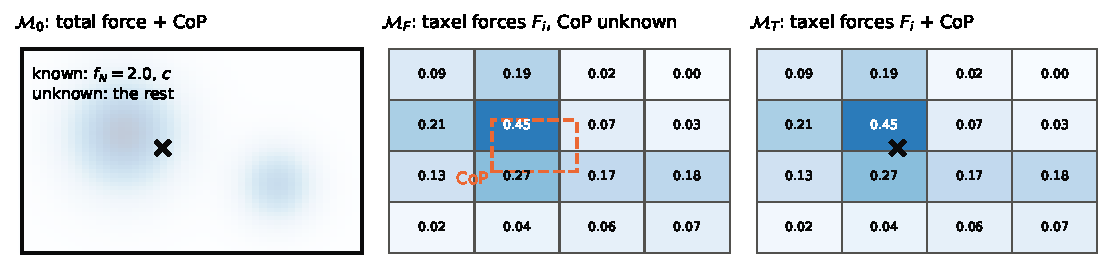
\includegraphics[width=\textwidth]{measurements}
    \caption{What each measurement operator observes for the same contact ($4\times4$ taxels). $\mathcal M_0$: only $f_N$ and the CoP, the pressure
    distribution (faded) is unknown. $\mathcal M_F$: the taxel forces $F_i$ (cells filled with the mean pressure $F_i/|P_i|$), the CoP is only known to lie
    in $\mathcal C_{\mathcal M_F}(y_F)$ (dashed, Proposition~\ref{prop:cop_taxel}). $\mathcal M_T$: taxel forces and CoP.
    }
    \label{fig:measurements}
\end{figure}
\begin{table}[t]
    \centering
    \small
    \resizebox{\textwidth}{!}{\begin{tabular}{lllll}
        \toprule
        Measurement & Observed data & Compatible CoP set & Lower bound & Upper bound \\
        \midrule
        $\mathcal M_0$ (Sec.~\ref{sec:M0})
        &
        $y_0=(f_N,f_Nc)$
        &
        $\{c\}$
        &
        closed form
        &
        LP (polygonal $P$)
        \\[1mm]
        $\mathcal M_T$ (Sec.~\ref{sec:MT})
        &
        $y_T=(y_0,y_F)$
        &
        $\{c\}$
        &
        convex (SOCP)
        &
        LP (polygonal taxels)
        \\[1mm]
        $\mathcal M_F$ (Sec.~\ref{sec:MF})
        &
        $y_F=(F_1,\ldots,F_r)$
        &
        $\displaystyle\sum_{i=1}^r\frac{F_i}{f_N}P_i$
        &
        convex (SOCP)
        &
        nonconvex: $\max_{c}$ of $\mathcal M_T$ LPs
        \\
        \bottomrule
    \end{tabular}}
    \caption{Measurement operators, compatible CoP sets and structure of the resulting bounds.}
    \label{tab:measurement_cases}
\end{table}
We next specialize \eqref{eq:general_nonlinear_lower}--\eqref{eq:general_nonlinear_upper} by increasing difficulty:
the CoP is first measured, with coarse (Section~\ref{sec:M0}) and then taxel-wise (Section~\ref{sec:MT}) force information.
It is then unknown (Section~\ref{sec:MF}). The tightening of the bounds as information is added is studied in Section~\ref{sec:refinement}.

\section{$\mathcal{M}_0$ case (coarse measurement)}
\label{sec:M0}

We first assume that the available measurements consist only of the resultant normal force $f_N$ and the CoP $c$.
\textcolor{blue}{\textbf{Known:} $P$, $\mu$, $f_N$ and $c$. \textbf{Unknown:} how $\nu_N^\star$ is distributed over $P$.}
Since the CoP is measured, Lemma~\ref{lem:cop_slicing} shows that both bounds are GMPs. We compute them explicitly and show
that this partial information is generally not enough to determine the admissible tangential wrench set.

\begin{definition}[Coarse normal force measurement]\label{def:coarse_measurement}
    Given the true (unknown) normal force measure $\nu_N^\star\in\mathcal M_+(P)$,
    we define the coarse measurement as its zeroth and first moments
    \begin{align}
    y_0 = \mathcal M_0(\nu_N^\star) \triangleq \left(\int_P d\nu_N^\star(x),\;\int_P x\,d\nu_N^\star(x)\right) = (f_N,f_Nc[\nu_N^\star])
    \end{align}
\end{definition}

\begin{remark}
    The coarse measurement $y_0=\mathcal M_0(\nu_N^\star)$ is a particular case of Definition~\ref{def:measurement_operator}, that extracts the zeroth and first moments through measurement functions:
    \begin{align}
        \phi_1(x)=1,\qquad
        \phi_2(x)=x_1,\qquad
        \phi_3(x)=x_2.
    \end{align}
    The set of compatible CoPs is the singleton $\mathcal C_{\mathcal M_0}(y_0)=\{c[\nu_N^\star]\}$.
\end{remark}

\begin{theorem}[Exact coarse lower bound]
\label{thm:coarse_lower}
    Let $c=c[\nu_N^\star]$. Given the coarse observation $y_0=(f_N, f_Nc)$, for any $q=(a,b)\in\mathbb R^2\times\mathbb R$,
    \begin{align}
            \boxed{\underline h_{\mathcal M_0}(q;y_0) = \mu f_N\|a\|_2}
    \end{align}
\end{theorem}
\begin{proof}
    By Lemma~\ref{lem:integrand}(iii), $h_{\mathcal W(\nu_N)}(q)\ge\mu f_N\|a\|_2$ for every $\nu_N\in\Pi_{\mathcal M_0}(y_0)$.
    Since $P$ is convex, $c\in P$, so $f_N\delta_c\in\Pi_{\mathcal M_0}(y_0)$, and it attains this value: the torque of a point load about its own
    location vanishes, so $\mathcal W(f_N\delta_c)=f_N B(0,\mu)\times\{0\}$.
\end{proof}

\begin{remark}
As an immediate consequence, setting $a=0$ shows that the coarse measurement does not guarantee any torsional capacity, i.e. $\underline h_{\mathcal M_0}((0,b);y_0)=0$.
\end{remark}

\begin{theorem}[Coarse upper bound]
\label{prop:coarse_upper_atomic}
    The supremum $\overline h_{\mathcal M_0}(q;y_0)$ is attained by a measure $\nu_N^+\in\Pi_{\mathcal M_0}(y_0)$ supported on at most three points, i.e.,
    \begin{align}
        \nu_N^+
        =
        \sum_{j=1}^{s}\lambda_j\delta_{x_j},
        \qquad s\leq 3,
    \end{align}
    where $x_j\in P$, $\lambda_j\geq 0$, and
    \begin{align}
        \sum_{j=1}^{s}\lambda_j=f_N,
        \qquad
        \sum_{j=1}^{s}\lambda_jx_j=f_Nc.
    \end{align}
\end{theorem}

\begin{proof}
    This is Proposition~4.4 of Yann's draft with the Coulomb set $C=B(0,\mu)$ (see Remark~\ref{rem:demontmarin}).
    There, as in~\cite{winkler1988extreme}, it follows from the fact that the extreme points of a set of measures defined by three linear moment
    constraints are supported on at most three points~\cite{lasserre2010moments}. \textcolor{red}{Check with Yann.}
    % A self-contained finite-dimensional argument is as follows.
    % On $\Pi_{\mathcal M_0}(y_0)$ the CoP is fixed to $c$, so the constraints and the objective depend on $\nu_N/f_N$ only through its moment vector
    % $\int_P\Phi\,d\nu_N/f_N$, with $\Phi(x)=(x,g(x;q,c))\in\R^3$, which lies in the compact convex set $K=\operatorname{conv}\Phi(P)$ (otherwise a separating plane gives a contradiction after integration).
    % The bound is therefore $\mu f_Nt^\star$, where $(c,t^\star)$ is the highest point of $K$ above $c$; it exists since $K$ contains the moment vector of $\nu_N^\star/f_N$.
    % This point lies on a supporting plane $H$ of $K$, and $K\cap H=\operatorname{conv}(\Phi(P)\cap H)$, so Carath\'eodory's theorem in the two-dimensional plane $H$
    % writes it as a convex combination $\sum_{j=1}^s\mu_j\Phi(x_j)$ with $s\le3$. The measure $f_N\sum_j\mu_j\delta_{x_j}$ belongs to $\Pi_{\mathcal M_0}(y_0)$ and attains the bound.
\end{proof}

\begin{corollary}[Polygonal contact patch]
\label{cor:coarse_upper_polygon}
    Under the assumptions of Theorem~\ref{prop:coarse_upper_atomic},suppose additionally that $P$ is a convex polygon
    with vertices $v_1,\ldots,v_K$. Then the coarse upper bound is given exactly by the linear program
    \begin{align}
    \boxed{
    \begin{aligned}
        \overline h_{\mathcal M_0}(q;y_0)
        =
        \mu\max_{\lambda_1,\ldots,\lambda_K}\quad&
        \sum_{k=1}^K
        \lambda_k\|a+bJ(v_k-c)\|_2\\
        \text{s.t.}\quad&
        \lambda_k\geq0,\qquad k=1,\ldots,K,\\
        &
        \sum_{k=1}^K\lambda_k=f_N,\\
        &
        \sum_{k=1}^K\lambda_kv_k=f_Nc.
    \end{aligned}}
    \end{align}
    Moreover, an optimal solution exists with
    at most three nonzero weights $\lambda_k$.
\end{corollary}

\begin{proof}
    By Theorem~\ref{prop:coarse_upper_atomic}, an optimal measure is $\sum_{j=1}^s\lambda_j\delta_{x_j}$ with $s\le3$. Write each $x_j$ as a convex
    combination $\sum_k\alpha_{jk}v_k$ of the vertices. Moving the mass $\lambda_j\alpha_{jk}$ from $x_j$ to $v_k$ preserves the zeroth and first moments
    and, by convexity of $g(\cdot;q,c)$ (Lemma~\ref{lem:integrand}(i)), does not decrease the objective. This is the reduction to the extreme points of $P$
    in Yann's Proposition~4.4. Hence an optimal measure supported on the vertices exists, which gives the LP. The LP has three equality
    constraints, so it has a basic optimal solution with at most three nonzero weights.
\end{proof}

\begin{remark}[Connection with Yann's formulation \textcolor{red}{To check with Yann}]
\label{rem:demontmarin}
    Theorem~\ref{prop:coarse_upper_atomic} and Corollary~\ref{cor:coarse_upper_polygon} are the Coulomb case $C=B(0,\mu)$ of Proposition~4.4 in
    Yann's draft, where the moment is taken about a fixed origin. 
    With his notation $x^\perp=-Jx$ and a twist $(\omega_N,v_T)$, his integrand is $s_C(\omega_Nx^\perp-v_T)=\mu\|v_T+\omega_NJx\|_2$, which equals $\mu\,g(x;q,c)$ for
    \begin{align*}
        b=\omega_N,\qquad a=v_T+\omega_NJc,
    \end{align*}
    % So the direction $(a,b)$ can be interpreted as the tangential velocity and spin?. 
    Yann's $D(c^\perp)$ collects the moment and tangential force generated by all
     distributions with CoP $c$, so that $f_N\,s_{D(c^\perp)}(-[\omega_N,v_T])=\overline h_{\mathcal M_0}(q;y_0)$
    %  (the sign of $q$ is irrelevant, since $g(x;-q,c)=g(x;q,c)$).
    A possible nice interpretation is that $h_{\mathcal W(\nu_N)}(q)$ is the maximal power dissipated by the twist
    (MDP) and $\overline h_{\mathcal M_0}$ is its worst case over the distributions compatible with $y_0$.
    % Proposition~\ref{prop:support} is the pointwise maximization used in his proof.
    % His finite program over at most three points of $P$, or of its extreme points, is
    % Theorem~\ref{prop:coarse_upper_atomic} and Corollary~\ref{cor:coarse_upper_polygon}. His special cases are Corollary~\ref{cor:M0_not_identifying}
    % (CoP at a vertex: a single point load) and $b=0$ (no spin: both bounds equal $\mu f_N\|a\|_2$). 
    % He also notes that $D(\cdot)$ is the natural place to add priors on the distribution; the taxel measurements of Sections~\ref{sec:taxels}--\ref{sec:MF} are such priors.
\end{remark}

The two bounds differ in general, which shows that the coarse measurement does not determine the admissible wrench set.

% \begin{corollary}[$\mathcal M_0(\nu_N)$ does not determine $\mathcal W(\nu_N)$]
% \label{cor:M0_not_identifying}
%     Let $y_0=(f_N,f_Nc)$. If $c$ is not an extreme point of $P$, there exist $\nu_N^{(1)},\nu_N^{(2)}\in\Pi_{\mathcal M_0}(y_0)$
%     with $\mathcal W(\nu_N^{(1)})\neq\mathcal W(\nu_N^{(2)})$, and
%     $\underline h_{\mathcal M_0}((0,b);y_0)=0<\overline h_{\mathcal M_0}((0,b);y_0)$ for every $b\neq0$.
%     If $c$ is an extreme point of $P$, then $\Pi_{\mathcal M_0}(y_0)=\{f_N\delta_c\}$ and $y_0$ determines $\mathcal W(\nu_N^\star)$.
% \end{corollary}
% \begin{proof}
%     If $c$ is not an extreme point, there is $u\neq0$ with $c\pm u\in P$. Let
%     $\nu_N^{(1)}=f_N\delta_c$ and $\nu_N^{(2)}=\frac{f_N}{2}(\delta_{c-u}+\delta_{c+u})$, both in $\Pi_{\mathcal M_0}(y_0)$. By Proposition~\ref{prop:support},
%     $h_{\mathcal W(\nu_N^{(1)})}((0,b))=0$ and $h_{\mathcal W(\nu_N^{(2)})}((0,b))=\mu|b|f_N\|u\|_2>0$.
%     Conversely, let $c$ be extreme and $\nu_N\in\Pi_{\mathcal M_0}(y_0)$ with $\nu_N\neq f_N\delta_c$. 
%     There is then a $B$ with $c\notin B$ and $\nu_N(B)>0$ (since $\nu_N(P)=f_N$, the measure $\nu_N$ must carry some force away
%     from $c$). 
%     If $\nu_N(B)=f_N$, the CoP $c$ of $\nu_N$ lies in $B$ (a convex set), which is a contradiction. Otherwise, split $\nu_N$ into the force carried by $B$
%     and the remainder: $\int_Px\,d\nu_N=\int_{B}x\,d\nu_N+\int_{P\setminus B}x\,d\nu_N$, with masses $\nu_N(B)$ and $f_N-\nu_N(B)$, both positive.
%     Writing each integral as its mass times its local CoP and dividing by $f_N$ gives $c=tc_B+(1-t)c'$ with
%     $t=\nu_N(B)/f_N\in(0,1)$, $c_B\in B\cap P$ the local CoP of the force carried by $B$, and $c'\in P$ the local CoP of the remainder (local CoPs lie in
%     the convex sets $B\cap P$ and $P$). Since $c\notin B$, $c_B\neq c$, and then also $c'\neq c$. Thus $c$ is a strict convex combination of two distinct
%     points of $P$, i.e., $c$ is not extreme, a contradiction.
% \end{proof}

\begin{example}[Segment patch]
\label{ex:segment}
    Let $P=[0,L]\times\{0\}$, $c=\left(\frac{L}{2},0\right)$, $\nu_N^{(1)}=f_N\delta_c$ and
    $\nu_N^{(2)}=\frac{f_N}{2}\delta_{(0,0)}+\frac{f_N}{2}\delta_{(L,0)}$. Both have
    $\mathcal M_0(\nu_N^{(1)})=\mathcal M_0(\nu_N^{(2)})=\left(f_N,f_N\left(\frac{L}{2},0\right)\right)$, but in the pure torsion direction
    $(a,b)=(0,1)$,
    \begin{align}
    h_{\mathcal W(\nu_N^{(1)})}(0,1)=0 ~~~\neq~~~ h_{\mathcal W(\nu_N^{(2)})}(0,1)=\mu f_N\frac{L}{2}=\overline h_{\mathcal M_0}((0,1);y_0).
    \end{align}
    % The last equality follows from Corollary~\ref{cor:coarse_upper_polygon}: the vertices are the endpoints and the LP has the single solution $\lambda_1=\lambda_2=\frac{f_N}{2}$.
\end{example}

The results of this section are recovered in Section~\ref{sec:MT} as the special case of a single taxel $P_1=P$.

\section{Taxel measurements: preliminaries (common setting)}
\label{sec:taxels}

We now assume that a tactile array measures the normal force carried by each taxel, with or without the coarse measurement.
This section fixes the setting and collects three lemmas used in Sections~\ref{sec:MT} and~\ref{sec:MF}.

\begin{assumption}[Taxel partition]
\label{ass:taxels}
    The patch $P$ is partitioned into $r$ nonempty, pairwise disjoint, convex Borel sets $P_1,\ldots,P_r$, called \textit{taxels},
    with $P=\bigcup_{i=1}^rP_i$. When stated, the closure of each taxel is a convex polygon
    $\overline{P_i}=\operatorname{conv}\{v_{i1},\ldots,v_{iK_i}\}$ with vertices $v_{ik}\in\R^2$.
\end{assumption}
% A grid of rectangular taxels, each with two closed and two open sides, satisfies Assumption~\ref{ass:taxels}.

\begin{definition}[Taxel force measurement]\label{def:MF}
    Given the true unknown normal force measure $\nu_N^\star$ and the partition $\{P_i\}_{i=1}^r$, the \textit{taxel force measurement} is defined as
    \begin{align}
    y_F = \mathcal M_F(\nu_N^\star) \triangleq
    \left(
    \nu_N^\star(P_1),\ldots,\nu_N^\star(P_r)
    \right).
    \end{align}
    Equivalently, its measurement functions are
    $\phi_i(x)=\mathbf 1_{P_i}(x)$, $i=1,\ldots,r$.
    The measured taxel forces are denoted  $F_i\triangleq\nu_N^\star(P_i)$, $i=1,\ldots,r$.
    Because in practice we can not tell to which of two neighboring taxels an edge load belongs, we call a measure compatible with $y_F$ if its force can be split among the taxel closures with the measured amounts:
    \begin{align}
        \label{eq:PiMF}
        \Pi_{\mathcal M_F}(y_F)\triangleq\Bigl\{\nu_N=\sum_{i=1}^r\nu_i:\ \nu_i\in\mathcal M_+(P)\text{ supported on }\overline{P_i},\ \nu_i(\overline{P_i})=F_i,\ i=1,\ldots,r\Bigr\}.
    \end{align}
\end{definition}
The set~\eqref{eq:PiMF} slightly enlarges the preimage $\mathcal M_F^{-1}(y_F)=\{\nu_N:\nu_N(P_i)=F_i\ \forall i\}$ (take $\nu_i$ the restriction of $\nu_N$ to $P_i$); in
particular it contains $\nu_N^\star$. The two sets differ only by loads on the taxel boundaries, which carry no force for a pressure density.
% and Remark~\ref{lem:closure} shows that they give the same bounds for rectangular taxels. 
In return, all the finite-dimensional formulas below hold with equality and
are attained, without any argument on the taxel boundaries. \textcolor{red}{To check with Yann}.

\begin{definition}[Combined coarse and taxel force measurement]
\label{def:MT}
If both coarse and taxel force information are available, we define the \textit{combined coarse-and-taxel measurement}
\begin{align}
    y_T=\mathcal M_T(\nu_N^\star)
    &\triangleq
    \bigl(
    \mathcal M_0(\nu_N^\star),
    \mathcal M_F(\nu_N^\star)
    \bigr) \\
    &= \left(
    (f_N,f_Nc[\nu_N^\star]), F_1,\ldots,F_r\right),
\end{align}
with compatible set $\Pi_{\mathcal M_T}(y_T)\triangleq\Pi_{\mathcal M_0}(y_0)\cap\Pi_{\mathcal M_F}(y_F)$.
\end{definition}

\begin{remark}[What is known]
     Since the taxels form a partition of $P$, $y_F$ determines the resultant normal force $f_N=m_0(\nu_N^\star) = \sum_{i=1}^r F_i$, and we assume $f_N>0$.
     In both cases, the patch, the partition, $\mu$ and the taxel forces $F_i$ are known, and the distribution of $\nu_N^\star$ inside each taxel is unknown.
     The CoP $c^\star=c[\nu_N^\star]$ is known under $\mathcal M_T$, but not determined by $y_F$ under $\mathcal M_F$. With a single taxel ($r=1$, $P_1=P$),
     $y_F=f_N$ and $\Pi_{\mathcal M_T}(y_T)=\Pi_{\mathcal M_0}(y_0)$: the coarse case is the single-taxel case of $\mathcal M_T$.
\end{remark}

\begin{lemma}[Local CoPs of the taxels]
\label{lem:taxel_barycenters}
    Under Assumption~\ref{ass:taxels}, let $\nu_N=\sum_i\nu_i\in\Pi_{\mathcal M_F}(y_F)$ be split as in~\eqref{eq:PiMF}, with $f_N=\sum_iF_i>0$. Define
    \begin{align}
        c_i \triangleq \begin{cases}
                            \frac{1}{F_i}\int x\,d\nu_i(x) \qquad &\text{if}~F_i >0\\
                            \text{any point in $\overline{P_i}$}~ \qquad &\text{if}~ F_i=0,
                        \end{cases}
    \end{align}
    i.e. $c_i$ is the local CoP of the normal force carried by taxel $i$. Then (i) $c_i\in\overline{P_i}$; (ii) $c[\nu_N]=\frac{1}{f_N}\sum_{i=1}^rF_ic_i$, i.e. the CoP is the $F_i$-weighted average of the local CoPs; (iii) for every $q$ and every $c\in\R^2$,
    \begin{align}
        \label{eq:taxel_jensen}
        \int_P g(x;q,c)\,d\nu_N(x)\ge\sum_{i=1}^rF_i\,g(c_i;q,c).
    \end{align}
    Conversely, for any $c_i\in\overline{P_i}$, the measure $\nu_N=\sum_{i=1}^rF_i\delta_{c_i}$ belongs to $\Pi_{\mathcal M_F}(y_F)$, has CoP
    $\frac{1}{f_N}\sum_iF_ic_i$, and equality holds in \eqref{eq:taxel_jensen}.
\end{lemma}
\begin{proof}
    (i) This is the same fact as $c\in P$ in the planar contact model (Lemma~4.1 of Yann's draft), applied to $\nu_i$: a weighted average of points of the
    closed convex set $\overline{P_i}$ stays in it. For a rectangular taxel this is immediate coordinate-wise: each coordinate of $c_i$ is an average of values
    in a closed interval, hence lies in it.
    (ii) $\int_Px\,d\nu_N=\sum_i\int x\,d\nu_i=\sum_iF_ic_i$.
    (iii) Lemma~\ref{lem:integrand}(iii) applied to each $\nu_i$ with $F_i>0$, summed over $i$.
    The converse follows by taking $\nu_i=F_i\delta_{c_i}$.
\end{proof}

\begin{proposition}[Compatible CoP set from taxel forces]
\label{prop:cop_taxel}
    Under Assumption~\ref{ass:taxels}, the set of CoPs compatible with a taxel force observation $y_F = (F_1,\ldots,F_r)$ is the weighted Minkowski sum
    \begin{align}
        \mathcal C_{\mathcal M_F}(y_F)
        =
        \left\{
        \frac{1}{f_N}
        \sum_{i=1}^r F_i c_i
        :
        c_i\in\overline{P_i},\quad i=1,\ldots,r
        \right\}
        =\sum_{i=1}^r\frac{F_i}{f_N}\overline{P_i},
    \end{align}
    which is compact and convex, and $\operatorname{diam} \mathcal C_{\mathcal M_F}(y_F)\le\frac{1}{f_N}\sum_{i=1}^r F_i\operatorname{diam}(P_i)\le\max_i\operatorname{diam}(P_i).$
\end{proposition}
\begin{proof}
    The inclusion $\subseteq$ follows from Lemma~\ref{lem:taxel_barycenters}(i)--(ii), and $\supseteq$ from its converse part.
    For the diameter, let $c=\frac{1}{f_N}\sum_iF_ic_i$ and $c'=\frac{1}{f_N}\sum_iF_ic_i'$ with $c_i,c_i'\in\overline{P_i}$. By the triangle inequality,
    \begin{align}
        \|c-c'\|_2
        \le
        \frac{1}{f_N}
        \sum_{i=1}^rF_i\|c_i-c_i'\|_2
        \le
        \frac{1}{f_N}
        \sum_{i=1}^rF_i\operatorname{diam}(P_i)
        \le
        \max_i\operatorname{diam}(P_i),
    \end{align}
    where the last inequality uses $F_i\ge0$ and $\sum_iF_i=f_N$.
\end{proof}

\begin{remark}[Intuition \textcolor{red}{Discuss with Yann}]
\label{rem:why_lemmas}
    In order to reduce infinite dimensional optimization over measures to finite dimensional optimization problems we need some lemmas/machinery (Figure~\ref{fig:vertex_reduction}).
    \begin{itemize}
        \item \textit{Lower bound = ``concentrate''.} Collapsing the force of each taxel onto its local CoP keeps $F_i$ and the CoP, and cannot
        increase the objective, since a bowl evaluated at an average point is below the average of the bowl (Jensen, Lemma~\ref{lem:taxel_barycenters}(iii)).
        One point per taxel suffices. Needed for all lower bounds, $\mathcal M_0$ (Theorem~\ref{thm:coarse_lower}, a single point at the CoP),
        $\mathcal M_T$ (Theorem~\ref{thm:combined_lower}) and $\mathcal M_F$ (Theorem~\ref{thm:taxel_lower}).
        \item \textit{Upper bound = ``spread to corners''.} Splitting a point load among the corners of its taxel, with weights whose average position is
        the load's position, keeps $F_i$ and the CoP, and cannot decrease the objective, since a bowl lies below its chords. Every compatible measure is thus
        dominated by an LP over corner weights (Lemma~\ref{lem:vertex_reduction}, proved by LP duality). This is Yann's reduction to the extreme points
        of the patch (Corollary~\ref{cor:coarse_upper_polygon}), applied taxel by taxel; Example~\ref{ex:segment} is the simplest instance. 
        Needed for all upper bounds, $\mathcal M_0$
        (Corollary~\ref{cor:coarse_upper_polygon}, corners of $P$), $\mathcal M_T$ (Theorem~\ref{thm:combined_upper}) and $\mathcal M_F$ (Theorem~\ref{thm:taxel_upper}).
        \item \textit{Boundaries.} A corner of a half open taxel may belong to its neighbor. In our model (Definition~\ref{def:MF}), a load on a shared edge or
        corner may be counted by either taxel, so corner-supported measures are admissible and all the finite-dimensional problems below are exact. See Remark~\ref{lem:closure}.
        % With a strict half-open convention they would be ``ghosts'' (Figure~\ref{fig:closure})
    \end{itemize}
\end{remark}

\begin{figure}[t]
    \centering
    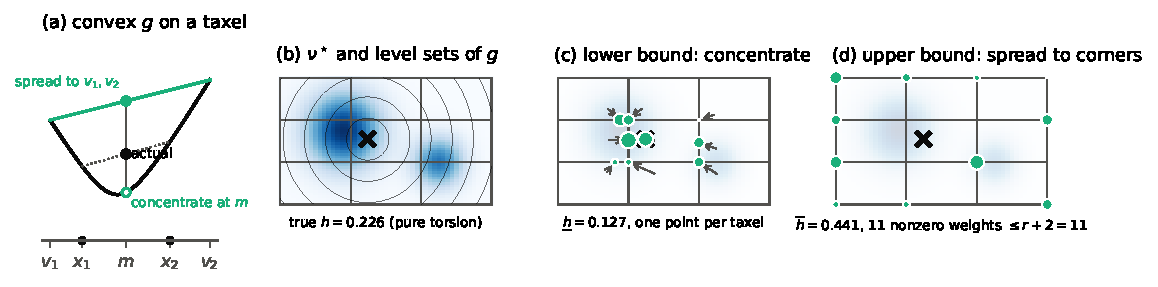
\includegraphics[width=\textwidth]{vertex_reduction}
    \caption{Concentrate vs.\ spread (Remark~\ref{rem:why_lemmas}), $3\times3$ taxels, pure torsion $q=(0,0,1)$, so $g(x;q,c)=\|x-c\|_2$.
    (a)~For masses at $x_1,x_2$ with CoP $m$: concentrating at $m$ lowers the objective (Jensen), spreading to the vertices
    $v_1,v_2$ raises it (chord). (b)~True measure and level sets of $g$. (c)~Minimizer of Theorem~\ref{thm:combined_lower}: one Dirac per
    taxel, pulled from the local CoPs of the taxels toward the CoP (arrows). (d)~Maximizer of Theorem~\ref{thm:combined_upper}: weights on the taxel
    corners, pushed away from the CoP, with at most $r+2$ nonzero weights. Marker areas are proportional to force.
    }
    \label{fig:vertex_reduction}
\end{figure}

\begin{lemma}[Vertex reduction]
\label{lem:vertex_reduction}
    Under Assumption~\ref{ass:taxels} with polygonal taxel closures, let $\nu_N=\sum_i\nu_i\in\Pi_{\mathcal M_F}(y_F)$, with $f_N=\sum_iF_i>0$ and
    $\int_Px\,d\nu_N(x)=f_Nc$. Then, for every $q$,
    \begin{align}
        \label{eq:vertex_reduction}
        \int_Pg(x;q,c)\,d\nu_N(x)\le V(q,c)\triangleq\max_{\lambda_{ik}\ge0}\left\{\sum_{i,k}\lambda_{ik}\,g(v_{ik};q,c):
        \sum_{k=1}^{K_i}\lambda_{ik}=F_i\ \forall i,\ \ \sum_{i,k}\lambda_{ik}v_{ik}=f_Nc\right\}.
    \end{align}
\end{lemma}
\begin{proof}
    We follow the idea of Yann's draft (Section~5.2) which uses the dual of the same LP for the whole patch (i.e., case $r=1$).
    \emph{The LP is feasible and bounded:} By Lemma~\ref{lem:taxel_barycenters}, the local CoPs $c_i\in\overline{P_i}$ satisfy $\sum_iF_ic_i=f_Nc$. Writing each $c_i$
    as a convex combination $\sum_k\alpha_{ik}v_{ik}$ of the corners of its taxel, $\lambda_{ik}=F_i\alpha_{ik}$ is feasible. The feasible set is compact, so the maximum exists.

    \emph{Dual LP:} With multipliers $y_i$ for the taxel constraints and $z\in\R^2$ for the CoP constraint, LP duality gives
    \begin{align*}
        V(q,c)=\min_{y\in\R^r,\,z\in\R^2}\left\{\sum_{i=1}^rF_iy_i+f_N\,z^\top c:\ y_i+z^\top v_{ik}\ge g(v_{ik};q,c)\ \forall i,k\right\}.
    \end{align*}

    \emph{Affine upper bound on each taxel:} Fix a dual-feasible $(y,z)$, and let $\ell_i(x)=y_i+z^\top x$. By the constraints, $\ell_i\ge g(\cdot;q,c)$ at the corners of $\overline{P_i}$.
    A convex function that lies below an affine one at the corners of a polygon lies below it on the whole polygon: for $x=\sum_k\alpha_kv_{ik}$,
    $g(x;q,c)\le\sum_k\alpha_kg(v_{ik};q,c)\le\sum_k\alpha_k\ell_i(v_{ik})=\ell_i(x)$ (Lemma~\ref{lem:integrand}(i)).

    \emph{Integrate:} Since $\nu_i$ carries $F_i$ on $\overline{P_i}$ and $\nu_N$ has first moment $f_Nc$,
    \begin{align*}
        \int_Pg(x;q,c)\,d\nu_N(x)=\sum_{i=1}^r\int g(x;q,c)\,d\nu_i(x)\le\sum_{i=1}^r\int\left(y_i+z^\top x\right)d\nu_i(x)=\sum_{i=1}^rF_iy_i+f_N\,z^\top c.
    \end{align*}
    Then we take the min over dual feasible $(y,z)$ and get~\eqref{eq:vertex_reduction}.
    % This is the ``spread to corners'' idea step of Remark~\ref{rem:why_lemmas} (and of Corollary~\ref{cor:coarse_upper_polygon})
\end{proof}

\begin{remark}[Strict half-open taxels]
\label{lem:closure}
    One could instead require $\nu_N(P_i)=F_i$ exactly, with the half-open taxels, i.e., use the preimage $\mathcal M_F^{-1}(y_F)\subseteq\Pi_{\mathcal M_F}(y_F)$.
    Our bounds are conservative for this stricter model (Lemma~\ref{lem:monotone}). If we adopted the stricte convention we could still construct some admissible distribution by pushing the corner points toward the interior in a way that does not affect the CoP (important for $\mathcal{M}_T$ which constrains it)?
    % (ii) For rectangular taxels they are equal. We construct, from any
    % $\nu_N=\sum_i\nu_i\in\Pi_{\mathcal M_T}(y_T)$, a strict measure $\nu_N^\varepsilon$ with the same taxel forces and CoP by pushing every mass of $\nu_i$ a fraction
    % $\varepsilon$ of the way toward a target point $p_i\in P_i$ (Figure~\ref{fig:closure}(b)). The targets average to the CoP, $\sum_iF_ip_i=f_Nc$: e.g., the local CoPs
    % of $\nu_N^\star$, which lie in the half-open taxels. Then every mass, including a ghost mass on a corner owned by a neighbor, is pulled into its own taxel
    % (for a rectangle this is coordinate-wise: a point of $[\alpha,\beta]$ moved toward a point of $[\alpha,\beta)$ ends in $[\alpha,\beta)$); the CoP does not move, since both the
    % old masses and the targets average to $c$; and each mass moves by at most $\varepsilon\operatorname{diam}(P_i)$, so the value changes by at most
    % $\varepsilon|b|\sum_iF_i\operatorname{diam}(P_i)$ (Lemma~\ref{lem:integrand}(ii)). Without a CoP constraint ($\mathcal M_F$), any targets $p_i\in P_i$ will do.
\end{remark}

% \begin{figure}[t]
%     \centering
%     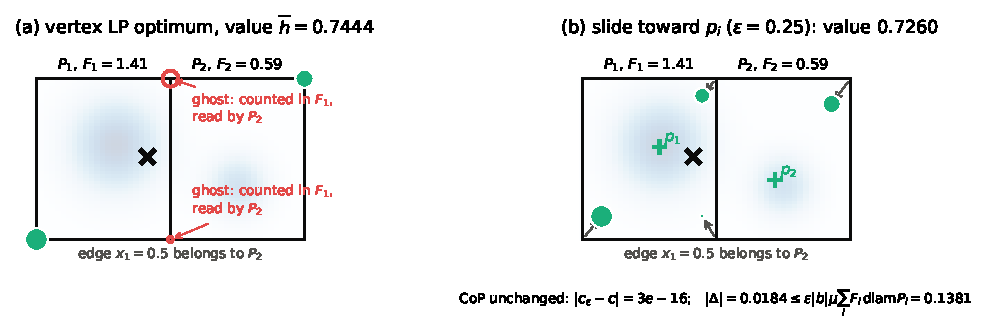
\includegraphics[width=\textwidth]{closure}
%     \caption{Ghost masses in the strict half-open model (Remark~\ref{lem:closure}), two half-open taxels, $\mathcal M_T$, direction $q=(0,1,1)/\sqrt2$
%     (rotation center $p$ to the left of the patch). (a)~The vertex LP of Theorem~\ref{thm:combined_upper} puts mass on the right corners of $P_1$,
%     which belong to $P_2$: with strict half-open taxels, no real load there would be read as $F_1$. (b)~Sliding every mass of $P_i$ a fraction $\varepsilon$ toward a
%     point $p_i\in P_i$ with $\sum_iF_ip_i=f_Nc$ (here, the local CoPs of the taxels for $\nu_N^\star$) gives a measure that is admissible even in the strict model, with exactly the same
%     CoP, whose value differs by at most $\varepsilon\mu|b|\sum_iF_i\operatorname{diam}(P_i)$. 
%     }
%     \label{fig:closure}
% \end{figure}


\section{$\mathcal{M}_T$ case (taxel forces with CoP)}
\label{sec:MT}

\textcolor{blue}{\textbf{Known:} the taxel forces $F_i$ and the CoP $c^\star=c[\nu_N^\star]$. \textbf{Unknown:} the distribution of $\nu_N^\star$ inside each taxel.}
Since $y_T$ determines the CoP, the set of compatible CoPs is reduced to a singleton $\mathcal C_{\mathcal M_T}(y_T)=\{c^\star\}$. Hence the outer optimization of
Lemma~\ref{lem:cop_slicing} disappears, and the $\mathcal M_T$-conditioned bounds reduce to the GMPs
    \begin{align}
    \underline h_{\mathcal M_T}(q;y_T)
    =
    \inf_{\substack{
    \nu_N\in\Pi_{\mathcal M_F}(y_F)\\
    \int_P(x-c^\star)\,d\nu_N=0}}
    \mu\int_P
    \|a+bJ(x-c^\star)\|_2\,d\nu_N(x),
\end{align}
\begin{align}
    \overline h_{\mathcal M_T}(q;y_T)
    =
    \sup_{\substack{
    \nu_N\in\Pi_{\mathcal M_F}(y_F)\\
    \int_P(x-c^\star)\,d\nu_N=0}}
    \mu\int_P
    \|a+bJ(x-c^\star)\|_2\,d\nu_N(x).
\end{align}
The taxel force constraints~\eqref{eq:PiMF} act on each taxel separately, but the CoP consistency constraint $\int_P(x-c^\star)\,d\nu_N=0$ couples the measure $\nu_N$ across the taxels.
In what follows, $c$ denotes the measured CoP $c^\star$.

\begin{theorem}[Exact lower bound for combined measurements]
\label{thm:combined_lower}
    Under Assumption~\ref{ass:taxels}, given the combined observation
    \begin{align}
        y_T
        &=
        \mathcal M_T(\nu_N^\star)
        =(y_0,y_F),\\
        y_0&=(f_N,f_Nc),
        \qquad
        y_F=(F_1,\ldots,F_r),
    \end{align}
    where $f_N=\sum_{i=1}^rF_i>0$, the measurement-conditioned
    lower bound satisfies
    \begin{align}
        \label{eq:combined_lower_reduction}
        \boxed{
        \begin{aligned}
        \underline h_{\mathcal M_T}(q;y_T)
        =
        \mu\min_{c_1,\ldots,c_r}\quad&
        \sum_{i=1}^r
        F_i\left\|a+bJ(c_i-c)\right\|_2\\
        \text{subject to}\quad&
        c_i\in\overline{P_i},
        \qquad i=1,\ldots,r,\\
        &
        \sum_{i=1}^rF_ic_i=f_Nc.
        \end{aligned}}
    \end{align}
    The resulting finite-dimensional optimization problem is convex, and an SOCP when the taxel closures are polygons.
\end{theorem}
\begin{proof}
    This is the ``concentrate'' step of Remark~\ref{rem:why_lemmas}.
    ($\ge$) For $\nu_N\in\Pi_{\mathcal M_T}(y_T)$, its local CoPs are feasible and $h_{\mathcal W(\nu_N)}(q)\ge\mu\sum_iF_i\,g(c_i;q,c)$, by Lemma~\ref{lem:taxel_barycenters}.
    ($\le$) For feasible $(c_i)$, the measure $\sum_iF_i\delta_{c_i}\in\Pi_{\mathcal M_T}(y_T)$ attains the objective (converse part of Lemma~\ref{lem:taxel_barycenters}).
    The minimum exists (compact feasible set, nonempty since $c\in\mathcal C_{\mathcal M_F}(y_F)$, continuous objective), and the problem is convex by
    Lemma~\ref{lem:integrand}(i), since the constraints are convex and affine. For polygonal closures, epigraph variables $t_i\ge\|a+bJ(c_i-c)\|_2$ give an SOCP.
\end{proof}

\begin{theorem}[Exact upper bound for combined measurements]
\label{thm:combined_upper}
    Under the assumptions of Theorem~\ref{thm:combined_lower},
    suppose additionally that each taxel closure is a polygon,
    \begin{align}
        \overline{P_i}
        =
        \operatorname{conv}
        \{v_{i1},\ldots,v_{iK_i}\},
    \end{align}
    where $v_{ik}\in\mathbb R^2$ are its vertices.
    Then, for every $q=(a,b)\in\mathbb R^2\times\mathbb R$,
    \begin{align}
        \label{eq:combined_upper_reduction}
        \boxed{
        \begin{aligned}
        \overline h_{\mathcal M_T}(q;y_T)
        =
        \mu\max_{\lambda_{ik}\geq0}\quad&
        \sum_{i=1}^r\sum_{k=1}^{K_i}
        \lambda_{ik}
        \left\|a+bJ(v_{ik}-c)\right\|_2\\
        \text{subject to}\quad&
        \sum_{k=1}^{K_i}\lambda_{ik}=F_i,
        \qquad i=1,\ldots,r,\\
        &
        \sum_{i=1}^r\sum_{k=1}^{K_i}
        \lambda_{ik}v_{ik}=f_Nc.
        \end{aligned}}
    \end{align}
    The resulting finite-dimensional optimization problem
    is a linear program, and an optimal solution exists with at most $r+2$ nonzero weights. In particular, the supremum is attained by a corner-supported measure.
\end{theorem}
\begin{proof}
    This is the ``spread to corners'' step of Remark~\ref{rem:why_lemmas}.
    ($\le$) For every $\nu_N\in\Pi_{\mathcal M_T}(y_T)$, $h_{\mathcal W(\nu_N)}(q)\le\mu V(q,c)$ by Lemma~\ref{lem:vertex_reduction}, and $V(q,c)$ is the LP \eqref{eq:combined_upper_reduction}.
    ($\ge$) For an optimal $\lambda$, the corner-supported measure $\sum_{i,k}\lambda_{ik}\delta_{v_{ik}}$ belongs to $\Pi_{\mathcal M_T}(y_T)$ (its piece on $\overline{P_i}$ is
    $\sum_k\lambda_{ik}\delta_{v_{ik}}$) and attains the LP value.
    The LP is feasible and bounded (proof of Lemma~\ref{lem:vertex_reduction}), and a basic optimal solution has at most as many nonzero entries as equality constraints, i.e., $r+2$.
\end{proof}

\begin{remark}[Recovering the coarse case]
    For a single taxel $P_1=P$, the constraint of \eqref{eq:combined_lower_reduction} forces $c_1=c$, and Theorem~\ref{thm:combined_lower} reduces to Theorem~\ref{thm:coarse_lower}.
    Theorem~\ref{thm:combined_upper} reduces to Corollary~\ref{cor:coarse_upper_polygon}, with $r+2=3$ nonzero weights.
\end{remark}

The exact $\mathcal M_T$-conditioned bounds retain both the taxel-force
constraints and the global first-moment constraint associated with the measured
CoP. Simpler bounds can be obtained by treating the taxels independently. For a reference point $c\in\R^2$ and $i=1,\ldots,r$, define
\begin{align}
g_i^{\min}(q;c)
&\triangleq
\min_{x\in\overline{P_i}}
\|a+bJ(x-c)\|_2,\\
g_i^{\max}(q;c)
&\triangleq
\max_{x\in\overline{P_i}}
\|a+bJ(x-c)\|_2.
\end{align}
For $b\neq0$, $a+bJ(x-c)=bJ(x-p)$ with $p=c+Ja/b$, the instantaneous center of rotation.
Hence $g_i^{\min}(q;c)=|b|\operatorname{dist}(p,P_i)$ and, for polygonal closures, $g_i^{\max}(q;c)=|b|\max_k\|v_{ik}-p\|_2$. For $b=0$, both equal $\|a\|_2$.

\begin{proposition}[Constructive cellwise support bounds]
\label{prop:cellwise}
Let $q=(a,b)\in\mathbb R^2\times\mathbb R$.
Then, for every $\nu_N\in\Pi_{\mathcal M_T}(y_T)$,
\begin{align}
\boxed{
\mu\sum_{i=1}^r
F_i g_i^{\min}(q;c^\star)
\le
h_{\mathcal W(\nu_N)}(q)
\le
\mu\sum_{i=1}^r
F_i g_i^{\max}(q;c^\star).
}
\end{align}
\end{proposition}

\begin{proof}
For every $x\in\overline{P_i}$,
\begin{align}
g_i^{\min}(q;c^\star)
\le
\|a+bJ(x-c^\star)\|_2
\le
g_i^{\max}(q;c^\star).
\end{align}
Write $\nu_N=\sum_i\nu_i$ as in~\eqref{eq:PiMF}. Since $\nu_i$ is nonnegative with mass $F_i$ on $\overline{P_i}$, integration against $\nu_i$ gives
\begin{align}
F_i g_i^{\min}(q;c^\star)
\le
\int
\|a+bJ(x-c^\star)\|_2\,d\nu_i(x)
\le
F_i g_i^{\max}(q;c^\star).
\end{align}
Summing over $i$ yields
\begin{align}
\sum_{i=1}^rF_i g_i^{\min}(q;c^\star)
\le
\int_P
\|a+bJ(x-c^\star)\|_2\,d\nu_N(x)
\le
\sum_{i=1}^rF_i g_i^{\max}(q;c^\star).
\end{align}
The result follows from Proposition~\ref{prop:support}.
\end{proof}

Consequently,
\begin{align}
\label{eq:cellwise_MT}
\boxed{
\mu\sum_{i=1}^r F_i g_i^{\min}(q;c^\star)
\le
\underline h_{\mathcal M_T}(q;y_T)
\le
\overline h_{\mathcal M_T}(q;y_T)
\le
\mu\sum_{i=1}^r F_i g_i^{\max}(q;c^\star).
}
\end{align}
These cellwise bounds are directly computable from the taxel forces, the
measured CoP, and the taxel geometry, but need not be sharp. In particular,
independently attaining the minimum or maximum within each taxel may violate
the global first-moment constraint contained in $\mathcal M_T$.

\section{$\mathcal{M}_F$ case (taxel forces without CoP)}
\label{sec:MF}

\textcolor{blue}{\textbf{Known:} the taxel forces $F_i$. \textbf{Unknown:} the CoP $c^\star$ and the distribution of $\nu_N^\star$ inside each taxel.}
Contrary to $y_0$ and $y_T$, the taxel force measurement $y_F$ does not determine the CoP. It only confines it to the convex set
$\mathcal C_{\mathcal M_F}(y_F)$ of Proposition~\ref{prop:cop_taxel}, which shrinks as the taxel partition is refined. The bounds therefore keep the
bi-level structure of Lemma~\ref{lem:cop_slicing}, and the inner problems are exactly the $\mathcal M_T$ problems of Section~\ref{sec:MT}.

\begin{proposition}[$\mathcal M_F$ as $\mathcal M_T$ with unknown CoP]
\label{prop:MF_as_MT}
    For $c\in\mathcal C_{\mathcal M_F}(y_F)$, let $y_T(c)\triangleq((f_N,f_Nc),y_F)$. Then
    $\Pi_{\mathcal M_F}(y_F)=\bigcup_{c\in\mathcal C_{\mathcal M_F}(y_F)}\Pi_{\mathcal M_T}(y_T(c))$, and for every $q$,
    \begin{align}
        \label{eq:MF_as_MT}
        \boxed{
        \underline h_{\mathcal M_F}(q;y_F)=\inf_{c\in\mathcal C_{\mathcal M_F}(y_F)}\underline h_{\mathcal M_T}(q;y_T(c)),
        \qquad
        \overline h_{\mathcal M_F}(q;y_F)=\sup_{c\in\mathcal C_{\mathcal M_F}(y_F)}\overline h_{\mathcal M_T}(q;y_T(c)).}
    \end{align}
\end{proposition}
\begin{proof}
    With the notation of Lemma~\ref{lem:cop_slicing}, $\Pi_{\mathcal M_F}(y_F;c)=\Pi_{\mathcal M_T}(y_T(c))$.
\end{proof}

Proposition~\ref{prop:MF_as_MT} is a nested problem: an outer optimization over the unknown CoP $c\in\mathcal C_{\mathcal M_F}(y_F)$, and inner $\mathcal M_T$ problems at each $c$
(Theorems~\ref{thm:combined_lower} and~\ref{thm:combined_upper}). For both bounds, the outer variable can be eliminated exactly: the CoP constraint of the inner problem
determines $c$ from the inner decision variables, as the CoP $\bar c$ of the candidate measure. This gives the single-level problems of Theorems~\ref{thm:taxel_lower}
and~\ref{thm:taxel_upper}. They differ in convexity: the lower bound is convex, the upper bound is generally not. For the upper bound, fixing $c$ gives back the LP
\eqref{eq:combined_upper_reduction}, so a possible numerical strategy is an outer search of LPs over $c\in\mathcal C_{\mathcal M_F}(y_F)$.

\begin{theorem}[Exact lower bound for taxel force measurements]
\label{thm:taxel_lower}
    Under Assumption~\ref{ass:taxels}, let $y_F=(F_1,\ldots,F_r)=\mathcal M_F(\nu_N^\star)$, where $F_i=\nu_N^\star(P_i)\geq 0$, and assume that
    $f_N=\sum_{i=1}^r F_i>0$. Then, for every $q=(a,b)\in\mathbb R^2\times\mathbb R$,
    \begin{align}
        \label{eq:taxel_lower_reduction}
        \boxed{\underline h_{\mathcal M_F}(q;y_F)
        =
        \mu
        \min_{\substack{c_i\in\overline{P_i}\\i=1,\ldots,r}}
        \sum_{i=1}^r
        F_i\left\|a+bJ(c_i-\bar c)\right\|_2}
    \end{align}
where     \begin{align}
        \bar c
        \triangleq
        \frac{1}{f_N}\sum_{i=1}^r F_i c_i
    \end{align}
    is the CoP of the candidate measure $\sum_iF_i\delta_{c_i}$. 
    This finite-dimensional optimization problem is convex, and an SOCP when the taxel closures are polygons.
\end{theorem}

\begin{proof}
    By \eqref{eq:MF_as_MT} and Theorem~\ref{thm:combined_lower}, minimizing \eqref{eq:combined_lower_reduction} jointly over $c\in\mathcal C_{\mathcal M_F}(y_F)$ and the $c_i$
    eliminates the constraint $\sum_iF_ic_i=f_Nc$, with $c=\bar c$. Equivalently, directly: for $\nu_N\in\Pi_{\mathcal M_F}(y_F)$, Lemma~\ref{lem:taxel_barycenters}
    with $c=c[\nu_N]=\bar c$ gives the inequality $\ge$, and the measures $\sum_iF_i\delta_{c_i}$ give the converse.

    Since $\bar c$ is affine in $(c_1,\ldots,c_r)$, the objective is convex. The minimum exists (compact feasible set, continuous objective), and for polygonal
    closures epigraph variables give an SOCP.
\end{proof}

\begin{theorem}[Exact upper bound for polygonal taxels]
\label{thm:taxel_upper}
    Under the assumptions of Theorem~\ref{thm:taxel_lower},
    suppose additionally that each taxel closure is a polygon $\overline{P_i} = \operatorname{conv}\{v_{i1},\ldots,v_{iK_i}\}$ where $v_{ik}\in\mathbb R^2$ are its vertices.
    Let $\lambda_{ik} \geq 0$ such that $\sum_{k=1}^{K_i}\lambda_{ik}=F_i$, define
    \begin{align}
        \bar c(\lambda)
        \triangleq
        \frac{1}{f_N}
        \sum_{i=1}^r\sum_{k=1}^{K_i}
        \lambda_{ik}v_{ik},
    \end{align}
    the CoP of the candidate measure $\sum_{i,k}\lambda_{ik}\delta_{v_{ik}}$ (again a function of the decision variables, not a measurement).
    Then, for every $q=(a,b)\in\mathbb R^2\times\mathbb R$,
    \begin{align}
        \label{eq:taxel_upper_reduction}
        \boxed{
        \begin{aligned}
        \overline h_{\mathcal M_F}(q;y_F)
        =
        \mu\max_{\lambda_{ik}\geq0}\quad&
        \sum_{i=1}^r\sum_{k=1}^{K_i}
        \lambda_{ik}
        \left\|
        a+bJ\bigl(v_{ik}-\bar c(\lambda)\bigr)
        \right\|_2\\
        \text{subject to}\quad&
        \sum_{k=1}^{K_i}\lambda_{ik}=F_i,
        \qquad i=1,\ldots,r.
        \end{aligned}}
    \end{align}
    This single-level problem is generally nonconvex: the weights $\lambda_{ik}$ multiply norms that depend on $\lambda$ through $\bar c(\lambda)$.
    Fixing $c=\bar c(\lambda)$ turns it into the LP \eqref{eq:combined_upper_reduction}, so $\overline h_{\mathcal M_F}(q;y_F)$ is the maximum over
    $c\in\mathcal C_{\mathcal M_F}(y_F)$ of this LP. A finite sweep over $c$ therefore gives a value $\le\overline h_{\mathcal M_F}(q;y_F)$, which is not certified;
    Proposition~\ref{prop:fixed_ref} gives a certified value $\ge\overline h_{\mathcal M_F}(q;y_F)$.
\end{theorem}

\begin{proof}
    ($\le$) For $\nu_N\in\Pi_{\mathcal M_F}(y_F)$ with CoP $c=c[\nu_N]$, Lemma~\ref{lem:vertex_reduction} gives $h_{\mathcal W(\nu_N)}(q)\le\mu V(q,c)$, and every $\lambda$
    feasible for $V(q,c)$ is feasible for \eqref{eq:taxel_upper_reduction}, with $\bar c(\lambda)=c$.
    ($\ge$) For feasible $\lambda$, the corner-supported measure $\sum_{i,k}\lambda_{ik}\delta_{v_{ik}}$ belongs to $\Pi_{\mathcal M_F}(y_F)$, has CoP $\bar c(\lambda)$, and attains
    the objective of $\lambda$.
    The maximum exists, since the feasible set is compact and the objective continuous.
    Finally, grouping the feasible $\lambda$ by the value of $\bar c(\lambda)\in\sum_i\frac{F_i}{f_N}\overline{P_i}=\mathcal C_{\mathcal M_F}(y_F)$ (Proposition~\ref{prop:cop_taxel})
    gives the equivalent form, i.e., Proposition~\ref{prop:MF_as_MT} with the LP \eqref{eq:combined_upper_reduction} as inner problem.
\end{proof}

\paragraph{Fixed-reference bounds.}
In practice, an estimate $\hat c$ of the CoP is often available. It can be used in two different ways. \emph{Fixing the CoP}, i.e., imposing
$\int_P(x-\hat c)\,d\nu_N=0$, gives a single $\mathcal M_T$ problem; this is valid only if $\hat c$ is the true CoP, and otherwise it is just one slice of
Proposition~\ref{prop:MF_as_MT}. \emph{Fixing the reference} instead means using $\hat c$ only as the point about which the torque is computed, without
enforcing the CoP constraint. In that case, the taxel constraints are
independent and the optimization decouples into the cellwise quantities of Section~\ref{sec:MT}:
\begin{align}
\underline h_F^{\mathrm{ref}}(q;y_F,\hat c)
=
\mu\sum_{i=1}^r
F_i\,g_i^{\min}(q;\hat c),
\qquad
\overline h_F^{\mathrm{ref}}(q;y_F,\hat c)
=
\mu\sum_{i=1}^r
F_i\,g_i^{\max}(q;\hat c).
\end{align}
These expressions are not bounds for the $\mathcal M_F$-conditioned problem, because the true CoP differs from $\hat c$. They become bounds after a correction for the uncertainty of the CoP.

\begin{proposition}[Certified fixed-reference bounds]
\label{prop:fixed_ref}
    For every $\hat c\in\R^2$, let $\delta(\hat c)\triangleq\sup_{c\in\mathcal C_{\mathcal M_F}(y_F)}\|c-\hat c\|_2$. Then, for every $q=(a,b)$,
    \begin{align}
        \underline h_F^{\mathrm{ref}}(q;y_F,\hat c)-\mu|b|f_N\delta(\hat c)
        \le
        \underline h_{\mathcal M_F}(q;y_F)
        \le
        \overline h_{\mathcal M_F}(q;y_F)
        \le
        \overline h_F^{\mathrm{ref}}(q;y_F,\hat c)+\mu|b|f_N\delta(\hat c).
    \end{align}
    For $\hat c\in\mathcal C_{\mathcal M_F}(y_F)$, $\delta(\hat c)\le\operatorname{diam}\mathcal C_{\mathcal M_F}(y_F)$.
\end{proposition}
\begin{proof}
    Let $\nu_N\in\Pi_{\mathcal M_F}(y_F)$ with $c=c[\nu_N]\in\mathcal C_{\mathcal M_F}(y_F)$. By Lemma~\ref{lem:integrand}(ii),
    $|g(x;q,c)-g(x;q,\hat c)|\le|b|\delta(\hat c)$, so
    $\left|h_{\mathcal W(\nu_N)}(q)-\mu\int_Pg(x;q,\hat c)\,d\nu_N\right|\le\mu|b|f_N\delta(\hat c)$.
    The cellwise argument of Proposition~\ref{prop:cellwise}, applied with reference $\hat c$, bounds $\mu\int_Pg(x;q,\hat c)\,d\nu_N$ between
    $\underline h_F^{\mathrm{ref}}$ and $\overline h_F^{\mathrm{ref}}$.
\end{proof}

\begin{remark}[Using an estimate of the CoP]
\label{rem:cop_estimate}
    The correction $\delta(\hat c)$ is a supremum over all of $\mathcal C_{\mathcal M_F}(y_F)$, so a more accurate $\hat c$ does not reduce it by itself; it is smallest
    when $\hat c$ is the centre of $\mathcal C_{\mathcal M_F}(y_F)$. If additional information guarantees that the true CoP lies in a subset
    $\mathcal C\subseteq\mathcal C_{\mathcal M_F}(y_F)$ (e.g. an estimate with a known error radius), the same proof applies to the measures with CoP in $\mathcal C$,
    with $\delta(\hat c)$ taken over $\mathcal C$. For the upper bound, Proposition~\ref{prop:fixed_ref} avoids the nonconvex problem of
    Theorem~\ref{thm:taxel_upper}. The exact upper bound is then bracketed: the best value found by a finite sweep over $c\in\mathcal C_{\mathcal M_F}(y_F)$ of the LP
    \eqref{eq:combined_upper_reduction} is $\le\overline h_{\mathcal M_F}(q;y_F)\le\overline h_F^{\mathrm{ref}}(q;y_F,\hat c)+\mu|b|f_N\delta(\hat c)$.
    For the lower bound, Theorem~\ref{thm:taxel_lower} is already a single convex program and at least as tight, so an estimate of the CoP is not needed there.
\end{remark}

% \begin{remark}[Reference point of the torque]
% \label{rem:reference_point}
%     The fixed-reference quantities are exact bounds for a different wrench: the torque taken about the fixed point $\hat c$ instead of the CoP.
%     Indeed, $\tau_{\hat c}=\int_P(x-\hat c)\times\gamma_T\,d\nu_N=\tau_N+(c[\nu_N]-\hat c)\times f_T$, and the support function of the corresponding wrench set is
%     $\mu\int_Pg(x;q,\hat c)\,d\nu_N(x)$. Its integrand no longer depends on $c[\nu_N]$, so the problem over $\Pi_{\mathcal M_F}(y_F)$ is a GMP with only the
%     taxel constraints, and it decouples: its infimum and supremum are $\underline h_F^{\mathrm{ref}}$ and $\overline h_F^{\mathrm{ref}}$. Hence the nonconvexity in
%     Theorem~\ref{thm:taxel_upper} comes only from measuring the torsion about the unknown CoP; the term $\mu|b|f_N\delta(\hat c)$ of Proposition~\ref{prop:fixed_ref}
%     is the price of moving the reference point back to it. In Yann's draft, where the twist is expressed about a fixed origin, the same structure
%     appears as the concavity of $a\mapsto s_{D(a)}$ in his Proposition~4.4.
% \end{remark}

\section{Comparison of measurements and tightening under refinement}
\label{sec:refinement}

All results of this section follow from Lemma~\ref{lem:monotone} (inclusion of compatible families) and from the Lipschitz
property of Lemma~\ref{lem:integrand}(ii).

\begin{proposition}[Comparison of coarse, taxel and combined measurements]
\label{prop:taxel_refinement}
The compatible measure family associated with the combined measurement is
\begin{align}
\Pi_{\mathcal M_T}(y_T)
=
\Pi_{\mathcal M_0}(y_0)
\cap
\Pi_{\mathcal M_F}(y_F).
\end{align}
Consequently, for every wrench direction
$q\in\mathbb R^2\times\mathbb R$,
\begin{align}
\boxed{
\mu f_N\|a\|_2
=
\underline h_{\mathcal M_0}(q;y_0)
\le
\underline h_{\mathcal M_F}(q;y_F)
\le
\underline h_{\mathcal M_T}(q;y_T)
\le
h_{\mathcal W(\nu_N^\star)}(q)
}
\end{align}
and
\begin{align}
\boxed{
h_{\mathcal W(\nu_N^\star)}(q)
\le
\overline h_{\mathcal M_T}(q;y_T)
\le
\min\left\{
\overline h_{\mathcal M_0}(q;y_0),
\overline h_{\mathcal M_F}(q;y_F)
\right\}.
}
\end{align}
Thus, $\mathcal M_T$ provides bounds that are at least as tight as those
obtained from either $\mathcal M_0$ or $\mathcal M_F$ alone. The lower bounds of $\mathcal M_0$ and $\mathcal M_F$ are ordered,
whereas their upper bounds are not in general ordered.
\end{proposition}
\begin{proof}
    The identity follows from $y_T=(y_0,y_F)$, and the inequalities involving $\mathcal M_T$ from Lemma~\ref{lem:monotone}.
    Every $\nu_N\in\Pi_{\mathcal M_F}(y_F)$ has total mass $f_N$, so \eqref{eq:universal_lower} gives $\underline h_{\mathcal M_F}(q;y_F)\ge\mu f_N\|a\|_2=\underline h_{\mathcal M_0}(q;y_0)$
    (Theorem~\ref{thm:coarse_lower}). For the upper bounds, with a single taxel $\Pi_{\mathcal M_F}(y_F)\supseteq\Pi_{\mathcal M_0}(y_0)$, so $\overline h_{\mathcal M_F}\ge\overline h_{\mathcal M_0}$.
    For fine partitions, $\overline h_{\mathcal M_F}\to h_{\mathcal W(\nu_N^\star)}$ by Proposition~\ref{prop:taxel_resolution_MT}, which is generally smaller than $\overline h_{\mathcal M_0}$ (Corollary~\ref{cor:M0_not_identifying}).
\end{proof}

\begin{proposition}[Tightening under taxel refinement]
\label{prop:taxel_refinement_MF}
Let $\mathcal M_F'$ and $\mathcal M_T'$ denote the taxel-force and combined measurements associated with a
partition $\{P_j'\}$ that refines the partition $\{P_i\}$ associated with $\mathcal M_F$ and $\mathcal M_T$
(each $P_i$ is a union of cells $P_j'$), and let
\begin{align}
y_F=\mathcal M_F(\nu_N^\star),
\quad
y_F'=\mathcal M_F'(\nu_N^\star),
\quad
y_T=\mathcal M_T(\nu_N^\star),
\quad
y_T'=\mathcal M_T'(\nu_N^\star).
\end{align}
Then
\begin{align}
\Pi_{\mathcal M_F'}(y_F')
\subseteq
\Pi_{\mathcal M_F}(y_F),
\qquad
\Pi_{\mathcal M_T'}(y_T')
\subseteq
\Pi_{\mathcal M_T}(y_T),
\qquad
\mathcal C_{\mathcal M_F'}(y_F')
\subseteq
\mathcal C_{\mathcal M_F}(y_F).
\end{align}
Consequently, for every $q\in\mathbb R^2\times\mathbb R$ and $\mathcal M\in\{\mathcal M_F,\mathcal M_T\}$, with $y$ and $y'$ the corresponding observations,
\begin{align}
\boxed{
\underline h_{\mathcal M}(q;y)
\le
\underline h_{\mathcal M'}(q;y')
\le
h_{\mathcal W(\nu_N^\star)}(q)
\le
\overline h_{\mathcal M'}(q;y')
\le
\overline h_{\mathcal M}(q;y).
}
\end{align}
\end{proposition}
\begin{proof}
    If $\nu_N=\sum_j\nu_j'\in\Pi_{\mathcal M_F'}(y_F')$, grouping the pieces inside each taxel, $\nu_i=\sum_{j:P_j'\subseteq P_i}\nu_j'$, gives measures supported on
    $\overline{P_i}$ with mass $\sum_{j:P_j'\subseteq P_i}\nu_N^\star(P_j')=F_i$, so $\nu_N\in\Pi_{\mathcal M_F}(y_F)$.
    Intersecting with $\Pi_{\mathcal M_0}(y_0)$ gives the inclusion for $\mathcal M_T$ (Proposition~\ref{prop:taxel_refinement}). Conclude with Lemma~\ref{lem:monotone}.
\end{proof}

The monotonicity above is associated with \textit{partition refinement}, not
with the number of taxels $r$ alone. The convergence below, on the other hand, only requires the taxel diameters to vanish.

\begin{proposition}[Resolution-dependent gap bounds]
\label{prop:taxel_resolution_MT}
For every $q=(a,b)\in\mathbb R^2\times\mathbb R$,
\begin{align}
\boxed{
0
\le
\overline h_{\mathcal M_T}(q;y_T)
-
\underline h_{\mathcal M_T}(q;y_T)
\le
\mu |b|
\sum_{i=1}^r
F_i\operatorname{diam}(P_i)
\le
\mu |b| f_N
\max_i\operatorname{diam}(P_i),
}
\end{align}
\begin{align}
\boxed{
0
\le
\overline h_{\mathcal M_F}(q;y_F)
-
\underline h_{\mathcal M_F}(q;y_F)
\le
2\mu |b|
\sum_{i=1}^r
F_i\operatorname{diam}(P_i)
\le
2\mu |b| f_N
\max_i\operatorname{diam}(P_i).
}
\end{align}
Hence, along any sequence of taxel partitions with
$\max_i\operatorname{diam}(P_i)\rightarrow0$,
\begin{align}
\underline h_{\mathcal M_F}(q;y_F),\
\underline h_{\mathcal M_T}(q;y_T),\
\overline h_{\mathcal M_T}(q;y_T),\
\overline h_{\mathcal M_F}(q;y_F)
\rightarrow
h_{\mathcal W(\nu_N^\star)}(q).
\end{align}
\end{proposition}
\begin{proof}
    $\mathcal M_T$: by \eqref{eq:cellwise_MT}, the gap is at most $\mu\sum_iF_i(g_i^{\max}-g_i^{\min})(q;c^\star)$, and
    $g_i^{\max}-g_i^{\min}\le|b|\operatorname{diam}(P_i)$ by Lemma~\ref{lem:integrand}(ii).
    $\mathcal M_F$: let $\nu_N,\nu_N'\in\Pi_{\mathcal M_F}(y_F)$, with CoPs $c,c'\in\mathcal C_{\mathcal M_F}(y_F)$. For $x,x'\in\overline{P_i}$, Lemma~\ref{lem:integrand}(ii) gives
    $g(x;q,c)-g(x';q,c')\le|b|\left(\operatorname{diam}(P_i)+\operatorname{diam}\mathcal C_{\mathcal M_F}(y_F)\right)$. Integrating against the pieces of $\nu_N$ and $\nu_N'$ on each taxel,
    \begin{align}
        h_{\mathcal W(\nu_N)}(q)-h_{\mathcal W(\nu_N')}(q)
        \le
        \mu|b|\left(\sum_{i=1}^rF_i\operatorname{diam}(P_i)+f_N\operatorname{diam}\mathcal C_{\mathcal M_F}(y_F)\right)
        \le
        2\mu|b|\sum_{i=1}^rF_i\operatorname{diam}(P_i),
    \end{align}
    by Proposition~\ref{prop:cop_taxel}. Take the supremum over $\nu_N$ and the infimum over $\nu_N'$.
    Convergence follows since $h_{\mathcal W(\nu_N^\star)}(q)$ lies between the bounds (Lemma~\ref{lem:monotone}).
\end{proof}

% \subsection{Current issues and open questions}

% The three cases differ in the role played by the CoP. With $\mathcal M_0$ and
% $\mathcal M_T$, the CoP is measured. The bounds are GMPs with explicit finite-dimensional forms: a convex lower bound and,
% for polygonal taxels, an LP upper bound. With $\mathcal M_F$, the CoP is an unknown confined to the compatible set
% $\mathcal C_{\mathcal M_F}(y_F)$, which contracts as the taxel partition is refined. The lower bound remains a single convex
% program, but the upper bound requires a nonconvex outer search over $\mathcal C_{\mathcal M_F}(y_F)$ of $\mathcal M_T$ linear programs.
% The main remaining questions concern
% (i) efficient global solution of the $\mathcal M_F$ upper bound, i.e. the structure of $c\mapsto\overline h_{\mathcal M_T}(q;y_T(c))$;
% (ii) the sharpness of the resolution-dependent bounds above (numerically, the gaps decrease linearly with $\max_i\operatorname{diam}(P_i)$, with constants below the bounds);
% and (iii) the additional tightening provided by the CoP constraint in $\mathcal M_T$ relative to $\mathcal M_F$, which appears small in numerical experiments.

\section{Certified load factor}
\label{sec:load_factor}

A controller does not need the bounds direction by direction. It needs to know whether a given load $w$ can be carried and, if not, by how much
the contact should be strengthened (e.g., by squeezing harder). This is a question about the ray $\{sw:s\ge0\}$: how far along it the guaranteed
set extends. This section shows that the answer is one convex program for the taxel measurements, without constructing the guaranteed set.

\paragraph{Fixed reference.}
The load acting on a grasped object is known about a point $o$ fixed to the object (or to the hand), not about the CoP, which is unknown under
$\mathcal M_F$. We therefore take the torque about a fixed point $o\in\R^2$.

\begin{definition}[Admissible tangential wrench set about a fixed point]
\label{def:wrench_fixed_ref}
    For $\nu_N\in\mathcal M_+(P)$ and $o\in\R^2$, let $\mathcal W_o(\nu_N)$ be the set of $(f_T,\tau_o)$ with
    $f_T=\int_P\gamma_T\,d\nu_N$ and $\tau_o=\int_P(x-o)\times\gamma_T(x)\,d\nu_N(x)$, over all measurable $\gamma_T$ with $\|\gamma_T\|_2\le\mu$ $\nu_N$-a.e.
    Since $\tau_o=\tau_N+(c[\nu_N]-o)\times f_T$, $\mathcal W_o(\nu_N)$ is the image of $\mathcal W(\nu_N)$ by an invertible linear map; in particular it is
    convex, compact and contains $0$, and $\mathcal W_{c[\nu_N]}(\nu_N)=\mathcal W(\nu_N)$. The proof of Proposition~\ref{prop:support}, with $c[\nu_N]$
    replaced by $o$, gives its support function
    \begin{align}
        h_{\mathcal W_o(\nu_N)}(q)=\mu\int_Pg(x;q,o)\,d\nu_N(x).
    \end{align}
    As in Definition~\ref{def:measurement_support_bounds} and Remark~\ref{rem:inner_outer}, we write
    \begin{align}
        \underline h^{\,o}_{\mathcal M}(q;y)\triangleq\inf_{\nu_N\in\Pi_{\mathcal M}(y)}h_{\mathcal W_o(\nu_N)}(q),
        \qquad
        \mathcal W_o^-(y)\triangleq\bigcap_{\nu_N\in\Pi_{\mathcal M}(y)}\mathcal W_o(\nu_N).
    \end{align}
\end{definition}

The integrand $g(x;q,o)$ does not depend on the CoP of $\nu_N$. The lower bounds are therefore GMPs for every measurement, and no outer
optimization over the compatible CoPs is needed (compare Proposition~\ref{prop:MF_as_MT}). Under $\mathcal M_T$, taking $o=c^\star$ gives back the
bounds of Section~\ref{sec:MT}.

\begin{lemma}[Fixed-reference lower bounds for taxel measurements]
\label{lem:fixed_ref_lower}
    Under Assumption~\ref{ass:taxels}, for every $q=(a,b)$ and $o\in\R^2$,
    \begin{align}
        \underline h^{\,o}_{\mathcal M_F}(q;y_F)=\mu\min_{\substack{c_i\in\overline{P_i}\\i=1,\ldots,r}}\sum_{i=1}^rF_i\left\|a+bJ(c_i-o)\right\|_2,
    \end{align}
    and $\underline h^{\,o}_{\mathcal M_T}(q;y_T)$ is the same minimum with the additional constraint $\sum_{i=1}^rF_ic_i=f_Nc$.
\end{lemma}
\begin{proof}
    ($\ge$) For a compatible $\nu_N$, its local CoPs are feasible (Lemma~\ref{lem:taxel_barycenters}(i)--(ii)), and
    Lemma~\ref{lem:taxel_barycenters}(iii) with $c=o$ bounds $\int_Pg(x;q,o)\,d\nu_N$ from below by the objective.
    ($\le$) For feasible $c_i$, $\sum_iF_i\delta_{c_i}$ is compatible and attains the objective (converse part of Lemma~\ref{lem:taxel_barycenters}).
    The minimum exists, since the feasible set is compact and nonempty ($c\in\mathcal C_{\mathcal M_F}(y_F)$ for $\mathcal M_T$) and the objective continuous.
\end{proof}

\begin{definition}[Load factor]
\label{def:load_factor}
    For a nonzero load $w=(f,\tau)\in\R^2\times\R$, expressed about $o$, the \textit{load factor} of $\nu_N$ is
    $s^\star_o(\nu_N;w)\triangleq\max\{s\ge0:\,sw\in\mathcal W_o(\nu_N)\}$, and the \textit{certified load factor} is
    \begin{align}
        \underline s_{\mathcal M}(w;y)\triangleq\inf_{\nu_N\in\Pi_{\mathcal M}(y)}s^\star_o(\nu_N;w).
    \end{align}
    The load $w$ is carried by every compatible measure if and only if $\underline s_{\mathcal M}(w;y)\ge1$. More generally, a contact whose normal
    force is scaled by $\lambda$ carries $w$ if $\lambda\,\underline s_{\mathcal M}(w;y)\ge1$, since $\mathcal W_o(\lambda\nu_N)=\lambda\mathcal W_o(\nu_N)$.
\end{definition}

\begin{proposition}[Certified load factor]
\label{prop:load_factor}
    Let $w=(f,\tau)\neq0$ and $o\in\R^2$.
    \begin{enumerate}[label=(\roman*)]
        \item For every measurement operator,
        \begin{align}
            \boxed{
            \underline s_{\mathcal M}(w;y)
            =\max\left\{s\ge0:\,sw\in\mathcal W_o^-(y)\right\}
            =\inf_{q:\,\langle q,w\rangle=1}\underline h^{\,o}_{\mathcal M}(q;y).}
        \end{align}
        \item Under Assumption~\ref{ass:taxels} with polygonal closures $\overline{P_i}=\{x:A_ix\le d_i\}$, for $\sigma\in\{-1,+1\}$ let
        \begin{align}
            \boxed{
            \begin{aligned}
            V_\sigma\triangleq\mu\inf_{a\in\R^2,\,b\in\R,\,u_i\in\R^2}\quad&\sum_{i=1}^rF_i\left\|a+J(u_i-b\,o)\right\|_2\\
            \text{subject to}\quad&a^\top f+b\tau=1,\qquad\sigma b\ge0,\\
            &\sigma\left(A_iu_i-b\,d_i\right)\le0,\qquad i=1,\ldots,r,\\
            &\textstyle\sum_{i=1}^rF_iu_i=b\,f_Nc\qquad(\mathcal M_T\text{ only}),
            \end{aligned}}
        \end{align}
        with $V_\sigma=+\infty$ if infeasible. Then $\underline s_{\mathcal M}(w;y)=\min\{V_{+1},V_{-1}\}$ for $\mathcal M\in\{\mathcal M_F,\mathcal M_T\}$,
        and each $V_\sigma$ is an SOCP.
        \item If $(a^\star,b^\star,u^\star)$ is optimal for the smaller of the two programs, let $c_i=u_i^\star/b^\star$ if $b^\star\neq0$, and let
        $(c_i)$ be any feasible point of Lemma~\ref{lem:fixed_ref_lower} otherwise. Then $\hat\nu_N=\sum_iF_i\delta_{c_i}$ is compatible and
        $s^\star_o(\hat\nu_N;w)=\underline s_{\mathcal M}(w;y)$: the certificate is attained by a compatible measure.
        \item (Several contacts.) Let $K$ contacts act on the same rigid object, with independent measurements $y_k$ of their normal force measures
        $\nu^k_N$, the same $\mu$, and patches identified with subsets of a common plane (common coordinates $x$, torques about the common normal). Assume
        that the wrench components out of this plane are balanced without friction. The load $w$ is then carried if $w\in\mathcal W_o(\nu^1_N)\oplus\cdots\oplus\mathcal W_o(\nu^K_N)$
        (Minkowski sum). The certified load factor of the grasp, the infimum over all compatible $(\nu^1_N,\ldots,\nu^K_N)$ of $\max\{s\ge0:sw\in\bigoplus_k\mathcal W_o(\nu^k_N)\}$, is
        \begin{align}
            \boxed{\underline s_{\mathrm{grasp}}(w)=\inf_{q:\,\langle q,w\rangle=1}\sum_{k=1}^K\underline h^{\,o}_{\mathcal M^k}(q;y_k),}
        \end{align}
        and (ii) holds with the objectives of the $K$ contacts summed, a shared $(a,b)$, and separate variables $u^k_i$.
        Since $\bigoplus_k\mathcal W^-_o(y_k)\subseteq\bigcap_{(\nu^k_N)}\bigoplus_k\mathcal W_o(\nu^k_N)$, this is at least the load factor of the sum of the
        guaranteed sets of the individual contacts.
    \end{enumerate}
\end{proposition}
\begin{proof}[Proof sketch]
    (i) Fix $\nu_N$. Since $\mathcal W_o(\nu_N)$ is convex, compact and contains $0$, $\{s\ge0:sw\in\mathcal W_o(\nu_N)\}=[0,s^\star_o(\nu_N;w)]$ with
    $s^\star_o<\infty$. Hence $sw\in\mathcal W_o^-(y)$ if and only if $s\le s^\star_o(\nu_N;w)$ for all compatible $\nu_N$, which gives the first equality.
    A closed convex set is the set of points satisfying $\langle q,\cdot\rangle\le h(q)$ for all $q$ \cite[Section~13]{rockafellar1970convex}. For
    $\langle q,w\rangle\le0$ this holds for every $s\ge0$, since $h_{\mathcal W_o(\nu_N)}\ge0$. Therefore
    $s^\star_o(\nu_N;w)=\inf_{\langle q,w\rangle>0}h_{\mathcal W_o(\nu_N)}(q)/\langle q,w\rangle=\inf_{\langle q,w\rangle=1}h_{\mathcal W_o(\nu_N)}(q)$ by positive homogeneity
    (the constraint set is nonempty since $w\neq0$). Exchanging the infima over $\nu_N$ and over $q$ gives the second equality.

    (ii) By (i) and Lemma~\ref{lem:fixed_ref_lower}, $\underline s_{\mathcal M}(w;y)$ is the infimum of $\mu\sum_iF_i\|a+bJ(c_i-o)\|_2$ jointly over $(a,b)$
    with $a^\top f+b\tau=1$ and over the feasible $c_i$. The objective is bilinear in $(b,c_i)$. Split the feasible set by the sign of $b$ and substitute $u_i=bc_i$.
    For $\sigma b>0$, this is a bijection between the feasible $c_i$ and the $u_i$ with $u_i/b\in\overline{P_i}$, i.e., $\sigma(A_iu_i-b\,d_i)\le0$, and
    $\sum_iF_iu_i=b\,f_Nc$. Moreover $bJ(c_i-o)=J(u_i-b\,o)$, so the objective is preserved. For $b=0$, the original objective is $\mu f_N\|a\|_2$ for every
    feasible $(c_i)$, and feasible points exist. In the new variables, $\sigma A_iu_i\le0$ forces $u_i=0$ because $\overline{P_i}$ is bounded, and the
    objective is again $\mu f_N\|a\|_2$. The objective is a sum of norms of affine functions and the constraints are linear, so epigraph variables give an SOCP.

    (iii) $\hat\nu_N$ is compatible (converse part of Lemma~\ref{lem:taxel_barycenters}). With $q^\star=(a^\star,b^\star)$, by (i),
    $s^\star_o(\hat\nu_N;w)\le h_{\mathcal W_o(\hat\nu_N)}(q^\star)=\mu\sum_iF_i\|a^\star+b^\star J(c_i-o)\|_2=\underline s_{\mathcal M}(w;y)\le s^\star_o(\hat\nu_N;w)$.

    (iv) For fixed measures, $\bigoplus_k\mathcal W_o(\nu^k_N)$ is convex, compact, contains $0$, and has support function $\sum_kh_{\mathcal W_o(\nu^k_N)}$.
    The argument of (i) applies. The compatible family is a product of the individual families, and the $k$-th term of the sum depends only on $\nu^k_N$,
    so for fixed $q$ the infimum of the sum is the sum of the infima. For the inclusion, if $w_k\in\mathcal W^-_o(y_k)$ for each $k$, then
    $w_k\in\mathcal W_o(\nu^k_N)$ for every compatible $\nu^k_N$, so $\sum_kw_k\in\bigoplus_k\mathcal W_o(\nu^k_N)$.
\end{proof}

\begin{remark}[On Proposition~\ref{prop:load_factor}]
\label{rem:load_factor}
    \begin{itemize}
        \item \textit{Why not a grid of directions.} $\underline h^{\,o}_{\mathcal M}(\cdot;y)$ is an infimum of convex functions of $q$, and is not convex in general.
        Minimizing it over a finite set of directions gives a value $\ge\underline s_{\mathcal M}(w;y)$, which may certify a load that is not guaranteed.
        Minimizing jointly over $q$ and the $c_i$, after the change of variables $u_i=bc_i$, gives the exact value as a convex program.
        \item \textit{Coarse case.} With a single taxel and $o=c$ ($\mathcal M_0$), the constraint forces $c_1=c$, and (ii) gives $\underline s=\mu f_N/\|f\|_2$
        if $\tau=0$ and $\underline s=0$ if $\tau\neq0$ (take $a=0$, $b=1/\tau$). The coarse measurement never certifies a torsional load (Theorem~\ref{thm:coarse_lower}).
        \item \textit{Taxel boundaries.} The value is exact for the compatible family~\eqref{eq:PiMF}, defined with the taxel closures. For the stricter
        preimage $\mathcal M_F^{-1}(y_F)$ it is a valid, possibly conservative, certificate (Lemma~\ref{lem:monotone}).
        \item \textit{Scope.} The certificate is quasi-static and applies to the measured state. In a feedback loop the load and the contact change between
        decisions, which requires a separate margin. In (iv), the assumption on the out-of-plane components matters: with a free object, offset normal
        forces at opposing contacts create a couple about an in-plane axis that must be balanced by friction, which the planar model does not account for.
    \end{itemize}
\end{remark}

\begin{thebibliography}{9}

\bibitem{evans2015measure}
L.~C. Evans and R.~F. Gariepy,
\newblock \emph{Measure Theory and Fine Properties of Functions},
\newblock Revised ed., CRC Press, Boca Raton, FL, 2015.

\bibitem{lasserre2010moments}
J.-B. Lasserre,
\newblock \emph{Moments, Positive Polynomials and Their Applications},
\newblock Imperial College Press Optimization Series, vol.~1,
Imperial College Press, London, 2010.

\bibitem{winkler1988extreme}
G.~Winkler,
\newblock ``Extreme points of moment sets,''
\newblock \emph{Mathematics of Operations Research},
vol.~13, no.~4, pp.~581--587, 1988.

\bibitem{rockafellar1970convex}
R.~T. Rockafellar,
\newblock \emph{Convex Analysis},
\newblock Princeton University Press, Princeton, NJ, 1970.

\end{thebibliography}
\end{document}
